\documentclass[aps,
                pra,  
                a4paper, 
                amsmath, 
                amssymb, 
                preprint,
                tightenlines,  
                amsfonts,
                nofootinbib,
                %onecolumn,
                notitlepage
            ]{revtex4-2}
\usepackage[utf8]{inputenc}
\usepackage{graphicx, subfig, rotating, float, hyperref}
\usepackage[rightcaption]{sidecap}

\begin{document}

%Title
\title{PHYS4420 Assignment:\\Analysis of x-ray sources within the $\omega$-Centauri globular cluster}

%Authors and Info
\author{Joseph Hocking}
\email{22876965@student.uwa.edu.au}
\noaffiliation

%Compilation Date
\date{\today}

\begin{center}
        
    \Large
    \textbf{PHYS4420 Assignment:\\Analysis of x-ray sources within the $\omega$-Centauri globular cluster}
        
    \vspace{1.5cm}
    \normalsize
    \textbf{Joseph Hocking\\22876965@student.uwa.edu.au}\\
    (Dated: \today)
\end{center}

\begin{center}
    %Abstract
    A data analysis of Chandra X-Ray observation of the $\omega$-Centauri globular cluster, ObsID 13726 and 13727, was replicated. The original study by S. Henleywillis et al. found 233 sources, and performed spectral fitting upon 14 of the brightest known members of the cluster. Of the 14, 13 were reidentified here, and spectral fitting was repeated. This fitting found somewhat similar parameters to the original study. Additionally, the parameters, although varying, are found to still be in support of some of the major conclusions of this study, namely, the identification of a CH star as a symbiotic star, and the large proportion of high $n_H$ CVs present in the source list, which may be due to the presence of magnetic CVs distorting the statistics of the brightest CVs.
\end{center}

\section{Introduction}
Globular clusters are broadly spherical group of stars on the order of $\sim10^5-10^6$ objects. The globular cluster NGC 5139, more commonly referred to as $\omega$-Centauri (from here on $\omega$ Cen) is a well known historical example of a globular cluster. It was first identified by Greek astronomers, who in the 2nd century AD wrongly classified it as a star. It wasn't until Edmond Halley in 1677, taking advantage of the recent invention of the telescope, discovered that it was in fact a non-stellar object, however it took a further 150 years before James Dunlop classified it as a globular cluster. It is unique in that it is the largest globular cluster known within the Milky Way, with a radius of $86\pm6$ly and an estimated mass of $(4.05\pm0.1)\times10^6M_{\odot}$, which, along with other evidence for an intermediate mass black hole in its core, leads some to argue that it may in fact be a remnant of a dwarf galaxy, swallowed by the much larger Milky Way.
\par
The main mechanism of internal cluster dynamical evolution is due to gravitational interaction between bodies. Statistically, one may derive an approximate rule for the \textit{relaxation time} of a globular cluster as follows\cite{Yan2008}:
\begin{equation}
    t_{relax}\approx\frac{0.1N}{\log{N}}t_{cross}
\end{equation}
Where $N$ is the number of stars in the cluster, and $t_{cross}$ is the crossing time of stars within the cluster. For the $\omega$ Cen cluster, the half mass relaxation time has been found to be relatively long, at $t_{relax}\approx 10Gyr$. This is significant as the cluster has an estimated age of $\sim 12Gyrs$, thus many of the dynamics within the clusters are similar to those that would occur just after formation. One may observe the effect of this relaxation time by examining the radial distribution (or rather independence) of mass-light ratio, that is, there is broadly an even distribution of high and low mass stars. Whereas in clusters that have evolved over several relation times, the high mass stars tend to migrate towards the center of the cluster\cite{Yan2008}.
\par
Another important concept to consider is the effective \textit{negative heat capacity} of a cluster. This is a by-product of the virial theorem within a self gravitating system. Conceptually, as a body in orbit loses energy, its orbit becomes tighter, and thus the body's speed will increase (making it ``hotter"). Additionally, just as in thermodynamic systems, weak gravitational interactions between stars begins to establish an equipartition of kinetic energy. This will ultimately mean stars of higher mass will slow down as they transfer speed to stars of lower mass. Thus a segregation is formed of high mass stars towards the core of the cluster and low mass towards the outside. Because of the negative heat capacity of the cluster, it's core will become denser and denser as time goes on, and relatively quickly resulting in \textit{core collapse}. An easy analogy can be made to the structure of a star, which would undergo gravitational collapse if it were not held at equilibrium by the radiation pressure from nuclear fusion. In the case of globular clusters, the bound energy of binary star systems provide the necessary energy to keep the cluster in equilibrium. When a binary system interacts with outside binaries, there is a chance for one object in the binary to lose energy to the outside object, which through it's negative heat capacity will speed the binary system up, staving off core collapse\footnote{In fact, a single standard mass binary system of two $0.7M_{\odot}$ stars are able to contain more binding energy than the entire cluster they are contained within}. This mechanism is able to extend the time before core collapse to $\sim 10t_{relax}$. It is also interesting to note that observations have showing that insufficient numbers of binaries could be formed through encounters, given the known density of globular cluster cores, and so the majority of these are likely to be primordial binaries (or systems that \textit{formed} as binaries).
\par
\begin{SCfigure}
    \caption{A description of the potential x-ray sources within the globular clusters\cite{Verbunt2004}}
    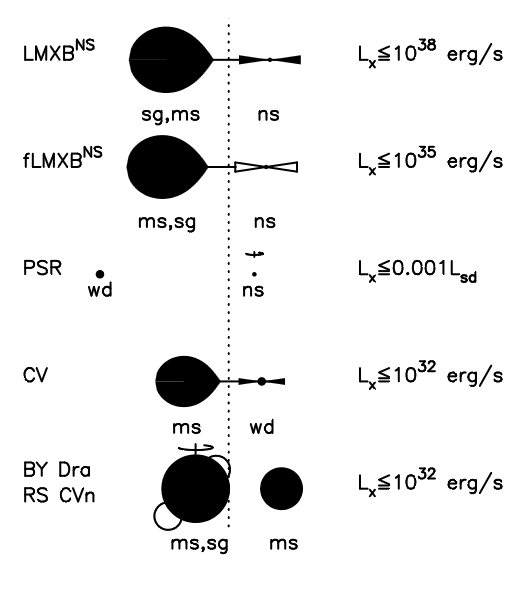
\includegraphics[width=0.4\textwidth]{img/gc-xray-sources.png}
    \label{fig:gc-xray-sources}
\end{SCfigure}
We can split x-ray sources in general into two categories: luminous and low-luminosity. Of the luminous sources with globular cluster, it is considered widely that they are all composed of binary systems of the type shown in Figure \ref{fig:gc-xray-sources}, and the CVs and CH (possible symbiotic) sources described in this analysis. Additionally the vast majority of low luminosity sources are of these same type or at the very least evolved from binary systems, however the red giant branch and sub giant branch stars (also identified in this analysis) are coronal sources likely from single stars. Given the relation to high luminosity x-ray sources and binaries, and given the importance of binary systems to the stability of globular clusters, studying x-ray sources within globular clusters is crucial to understanding cluster dynamics as a whole\cite{Verbunt2004,Henleywillis2018}. 
\par
The remainder of this report will be split up into 2 main sections: 1) Methodology and 2) Results. In the methodology section, there will be description of the observations and data processing pipeline, the source identification process, and the spectral extraction and fitting. The results section will be a discussion of the parameter estimation produced by the spectral fitting, and an interpretation of the values based off of known source identification.  

\section{Methodology}
\begin{figure}
    \centering
    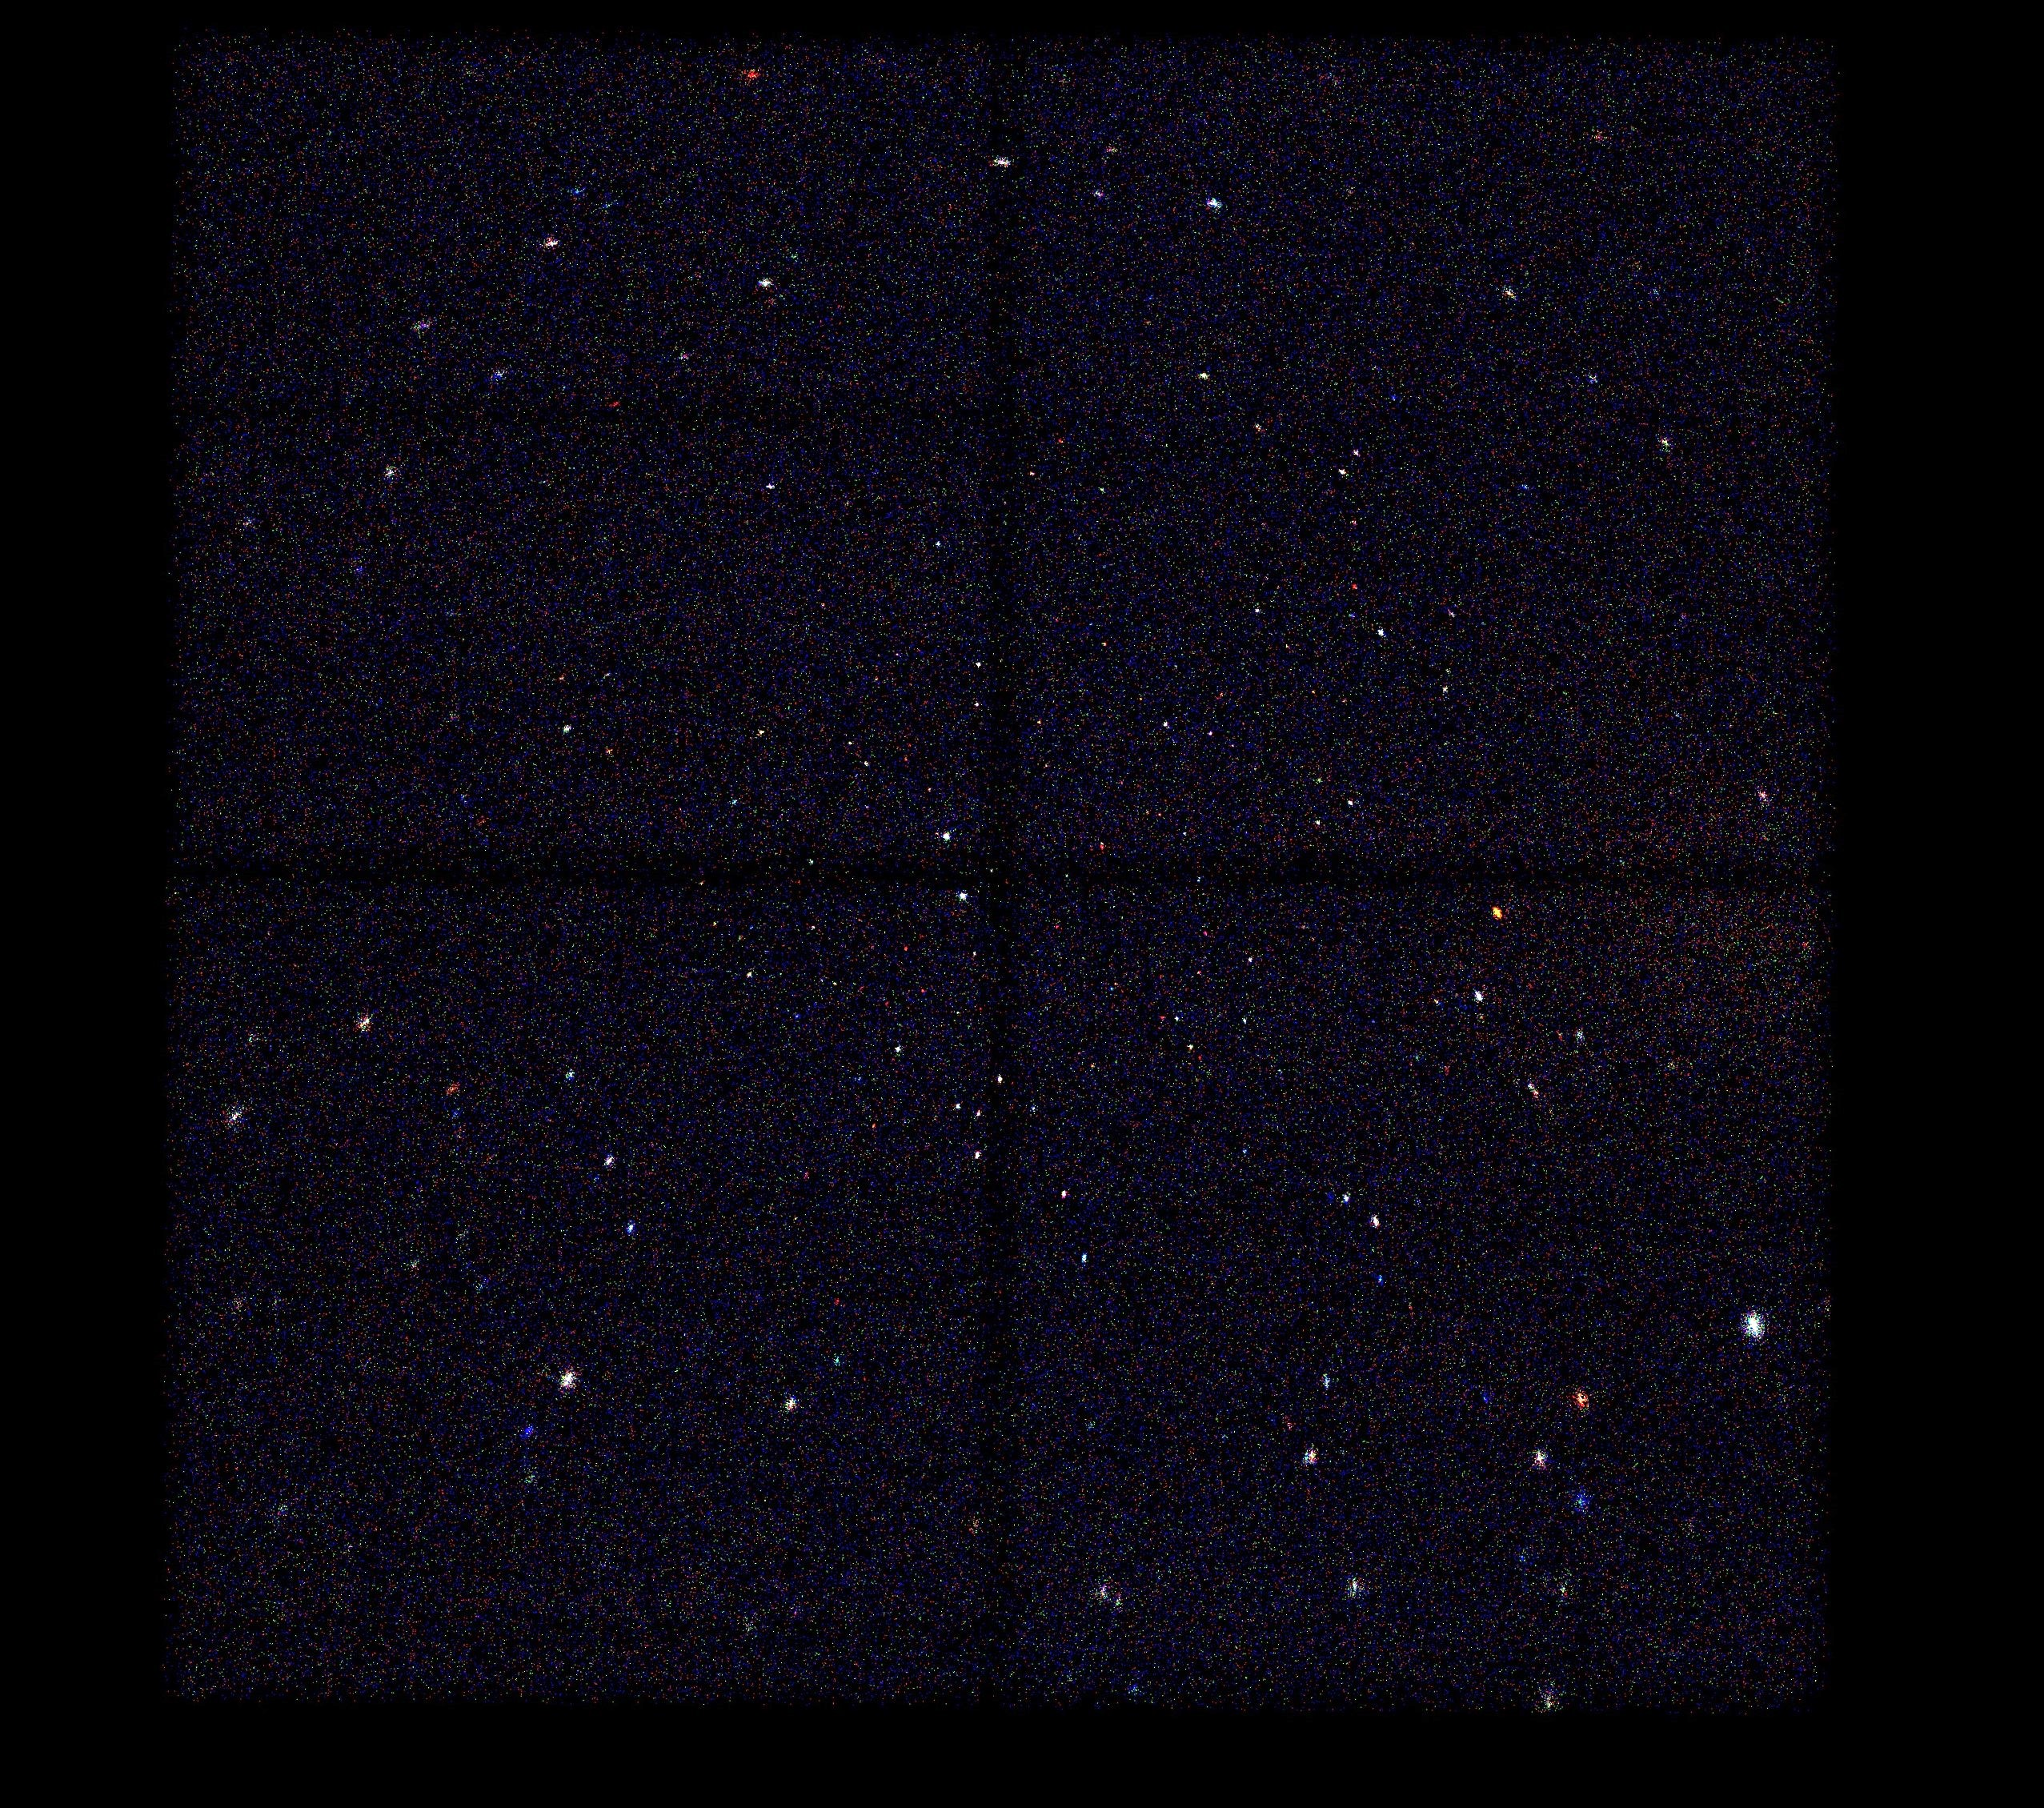
\includegraphics[width=0.85\textwidth]{img/truecolor-mx0.75-edit-bright.jpg}
    \caption{True color image of the $\omega$ Cen cluster as imaged by the ACIS-I CCD's from the merged observation files. This is composed of 3 energy bands, the soft x-ray (0.2-1.5 keV) is in red, the mid x-ray (1.5-2.5 keV) is in green, and the hard x-ray (2.5-8 keV) is in blue. The exposed image covers approximately 16.9x16.9 arcmin, with a resolution of ~0.49 arcsec/pixel. The four quadrants of the image are the 4 CCDs of the instrument, with each being 1024x1024 pixels, giving a total of 2048x2048 pixels for the image.}
    \label{fig:truecolor-picture}
\end{figure}

This analysis examined the same two datasets used by Henleywillis et. al. These were long-exposure time observations, one 173.7ks (ObsID 13726) and the other 48.5ks (ObsID 13727), of the $\omega$-Centauri globular cluster made with the {\it Chandra X-ray Observatory's} ACIS-I sensor. These observations, made in 2012, were targeted towards the detection of faint sources within the cluster, with more details on the set-up of the telescope in \cite{Henleywillis2018}. The processing and analysis (performed using the tools {\sc ciao} and {\sc xspec}) described herein will follow a very similar procedure as that used by Henleywillis et. al. To begin with, the two observations were reprocessed using {\sc chandra\_repro} as recommended by the documentation accompanying \textsc{ciao}. This tool accepts in the level 1 events files (that is, the raw data) and uses the most up-to-date calibration data appropriate for the observation to generate new level 2 event files. Before source-detection was performed, the reprocessed data files were then combined using the {\sc merge\_obs} tool, which also generated fluxed images, exposure maps, field-of-view files, and a merged point-spread function map (PSF). Henleywillis et al. generated these PSF maps outside of {\sc merge\_obs}, however, as the specified parameters are identical, this should not change the data files. These merged observations were limited to 0.5-4.5keV to reduce the background sources that could potentially be detected. The PSF maps were generated at 1.9keV and were merged by weighting the respective PSF maps for each observation by the exposure time. Additionally, an encircled counts fraction of 0.5 was selected. This was chosen to match the processing performed by Henleywillis et. al, who in turn found this value to give optimal source distinction. 
\par
The source detection was performed on the merged observation using the {\sc wavdetect} algorithm. Within {\sc ciao}, this works via a two step process: firstly, it performs a wavelet transform by correlating it with wavelet functions of the wavelet-scale sizes, and secondly a cell is generated around each source based off of the information from the wavelet transform. As per Henleywillis et al., wavelet scales of 1, 2, 4, and 8 were used, along with a significance threshold of $1e-06$ (this is the significance required for classifying a pixel as belonging to a source). In total, 240 sources were identified, many of which are likely background background sources. 
\par
To simplify the analysis, only the 14 of brightest sources (as in table 3 of Ref \cite{Henleywillis2018}) detected underwent spectral fitting. Not only did these sources benefit from having the highest counts, thus improving the fitting results, but also have previously been shown to be cluster members by Henleywillis et. al. To identify which of the detected sources corresponded with those described, {\sc dmcopy} was used to extract all detected sources above 70 counts in the 0.5-4.5keV band\footnote{Henleywillis et. al. used counts in the 0.5-6keV, this is likely with source 14 (73a) was missed}. Of the 14 sources sought after, 13 were detected, with the final source being 73a, which was the dimmest of the sources (the full source identification list is given in Table \ref{tab:fitting-results}). Regardless this was more than sufficient to continue on to the spectrum extraction of the sources. 
\par
Spectrum extraction was performed on each individual observation (ie. the level 2 event files as produced by {\sc chandra\_repro}) for the source regions identified. To do so, the {\sc .fits} region files outputted by {\sc wavdetect} were convert into ASCII{\sc .reg} files using {\sc dmmakereg}. These were then used to create a list (as a {\sc .lis} file) of virtual files, which each virtual file corresponding to a source region within the observation. Then the {\sc ciao} tool {\sc specextract} was ran on this list, with a few important parameters, namely the {\sc weight=no} essentially telling {\sc specextract} to treat the sources as point sources and to not spatially weight the auxiliary response files (ARF), and {\sc correctpsf=yes} which tells the tool to apply a point-source aperture correction to the {\it unweighted} ARF. This generated 26 spectra, 1 spectra for each source and each observation, along with additional response files. The spectra for each source from the two observations were then summed using the {\sc combine\_spectra} tool. 
\par
The script used to fit the spectra within {\sc xspec} and the compiled spectra files and fits maybe accessed online at \url{https://github.com/hockijo/4420-Omega-Cen-Data-Analysis/tree/main/chandra/CDRA/spec/new-spec}. Utilizing {\it C-statistics}\cite{Cash1979} to account for the low count numbers\footnote{This is based upon Poisson counting statistics, as opposed to the default $\chi^2$ based upon Gaussian statistics, this gives C-statistics a distinct advantage in the low count regimes.}. A {\sc tbabs*vmekal} model was used to fit to the data. {\sc tbabs}\cite{Wilms2000} is the Tuebingen-Boulder interstellar medium absorption model derived from Ref \cite{Wilms2000}. It accepts only the single parameter, $n_H$, the equivalent hydrogen column. {\sc vmekal}\cite{Mewe1985,Mewe1986,Liedahl1995} is a model for the emission from a hot, diffuse gas, including the emission lines from several elements. It accepts 19 parameters in total, with the free parameters being the temperature and a normalisation. The other parameters were the H density (fixed to $3\times10^{21}\text{cm}^{-2}$)\footnote{This was an estimation made after experimenting with the fitting parameters, it also coincides with an approximate middle value for the $n_H$ parameter given in Ref \cite{Henleywillis2018} Table 3 when excluding the high absorption sources.}, the abundances for the elements, (which were set to Solar abudance, excluding Fe, which was set to 0.03 Solar as per the [Fe/H]=-1.5 listed in \cite{Henleywillis2018}), the redshift (set to 0), and a switch parameter to tell the model to use emission lines from the AtomDB data. The equivalent hydrogen column for the {\sc tbabs} model had a lower bound of $9\times10^{20}\text{cm}^{-2}$, and was occasionally fixed at this value as shown in Table \ref{tab:fitting-results}. After fitting, 90\% confidence intervals for the free parameters were calculated using {\sc xspec}'s {\sc error} function, and a luminosity value in the 0.5-6keV band was calculated for each source using {\sc lumin}\footnote{This function required a non-zero redshift to be inputted, which was estimated from the distance to the globular cluster (5.2kPc\cite{Henleywillis2018}) and $H_0=70\text{km}\text{s}^{-1}\text{Mpc}^{-1}$, giving $z=d*H_0/c\approx1.2\times10^{-6}$}.

\section{Results and Discussion}
The fitted parameters, as well as other source information is given in Table \ref{tab:fitting-results}, and 4 of the more interesting spectra are shown in Fig \ref{fig:main-4-spectra}. Before examining specific sources, a few comments on the overall fitting are warranted. For the high luminosity sources, this analysis tended to underestimate when compared to the original. However, the uncertainty of the luminosities do overlap for the most part, suggesting that the difference may come down largely to statistical uncertainty. Also, for some best fit parameters (eg. source 4 temperature), the value was significantly larger than what was concluded previously. Additionally, the uncertainty on this parameter could not be calculated, as the {\sc error} function got stuck in an non-terminating loop. This leads to the conclusion that such parameters are unreliable and should not be used to compare previous results. Likely, the fitting was stuck inside a local minimum, however insufficient further analysis of the fitting would need to be performed to verify this. 
\vfill
\begin{center}
    \begin{sidewaystable}[ph!]
    \begin{tabular}{cccccccc}
        \hline
        Source ID & Ref \cite{Henleywillis2018} ID & Type & Position & Counts & $n_H$ & $kT$ & $L_x$\\
        & & & (RA[+201], DEC[-47]) & (0.5-4.5keV) & ($10^{20}$cm$^{-2}$) & (keV) & ($10^{30}$ ergs s$^{-1}$)\\
        \hline
        1 & 13c & CV & (0.7172$^{\pm3.7}$,0.4932$^{\pm2.7}$) & 2095(2042) & 12$^{+6}_{-\infty}$(16) & 49.1$^{+\infty}_{-29.2}$(34) & 537$^{+21}_{-24}$(570)\\
        2 & 13a & CV & (0.7123$^{\pm4.0}$,0.4834$^{\pm2.7}$) & 1924(1860) & 47$^{+13}_{-7}$(51) & 13.8$^{+8.3}_{-3.7}$(14.4) & 398$^{+18}_{-40}$(423)\\
        3 & 94a & CH & (0.5067$^{\pm32}$,0.5516$^{\pm27}$) & 1018(1088) & 41$^{+8}_{-9}$(72) & 24.0$^{+26.8}_{-10.1}$(6.8) & 368$^{+15}_{-13}$(466)\\
        4 & 54h & CV & (0.5849$^{\pm20}$,0.5008$^{\pm17}$) & 387(394) & 22$^{+16}_{-10}$(37) & 61.9$^{+\infty}_{-\infty}$(19.2) & 90$^{+20}_{-90}$(98)\\
        5 & 41d & CV & (0.6194$^{\pm14}$,0.4408$^{\pm9.5}$) & 363(360) & 94$^{+27}_{-23}$(112) & 17.7$^{+\infty}_{-9.1}$(14.6) & 117$^{+7}_{-54}$(117)\\
        6 & 43h & CV & (0.7066$^{\pm16}$,0.5368$^{\pm15}$) & 223(208) & 9$^{+13}_{-\infty}$(12) & 10.8$^{+16.2}_{-5.2}$(6.8) & 51$^{+1}_{-15}$(54)\\
        7 & 22c & fbCV & (0.7195$^{\pm11}$,0.4536$^{\pm7.7}$) & 180(179) & 9$^{+6}_{-\infty}$(11) & 5.6$^{+5.8}_{-1.9}$(5.7) & 31$^{+3}_{-7}$(39)\\
        8 & 11b & NV371 & (0.6707$^{\pm13}$,0.4604$^{\pm11}$) & 172(173) & 9$^{+\infty}_{-\infty}$(9) & 2.8$^{+1.1}_{-0.9}$(3.2) & 24$^{+1}_{-6}$(26)\\
        9 & 31a & fbCV & (0.6224$^{\pm20}$,0.4703$^{\pm15}$) & 120(119) & 18$^{+25}_{-\infty}$(21) & 25.3$^{+\infty}_{-19.9}$(22.3) & 27$^{+1}_{-27}$(27)\\
        10 & 54b & fbCV & (0.6770$^{\pm28}$,0.5525$^{\pm37}$) & 105(103) & 137$^{+69}_{-33}$(196) & 75.5$^{+\infty}_{-\infty}$(13.0) & 35$^{+35}_{-20}$(34)\\
        11 & 34b & RGB/SGB-a & (0.6560$^{\pm25}$,0.5147$^{\pm24}$) & 87(87) & 51$^{+36}_{-27}$(55) & 2.9$^{+2.6}_{-1.0}$(2.7) & 16$^{+2}_{-3}$(17)\\
        12 & 32f & RGB/SGB-a & (0.7723$^{\pm37}$,0.4691$^{\pm26}$) & 77(73) & 9*(9*) & 3.9$^{+5.6}_{-1.1}$(2.2) & 13$^{+1}_{-3}$(12)\\
        13 & 24c & CV & (0.6601$^{\pm22}$,0.5101$^{\pm15}$) & 72(71) & 9*(9*) & 6.4$^{+19.2}_{-3.1}$(5.7) & 12$^{+1}_{-3}$(12)\\
    \end{tabular}
    \caption{List of X-ray sources within $\omega$ Cen. The types are as described in Ref \cite{Henleywillis2018}. The positions were determined by the source detection algorithm in degrees (with the listed offset +201 and -47 for right ascension and declination respectively), and the uncertainty is given in ($10^{-6}$)$^\circ$. In the remaining columns, the value determined by this analysis is given, with the value from Ref \cite{Henleywillis2018} given in parentheses. The counts were determined automatically from {\sc wavdetect} and the uncorrected counts are given from Ref \cite{Henleywillis2018}. A * represents that the parameter was fixed during the fit. The $\infty$ in the uncertainty means that either the error calculation hit the lower and upper bound for the given parameter, or that the error calculation did not terminate.}
    \label{tab:fitting-results}
    \end{sidewaystable}
\end{center}

\begin{figure}[H]
    \centering
    \subfloat[][]{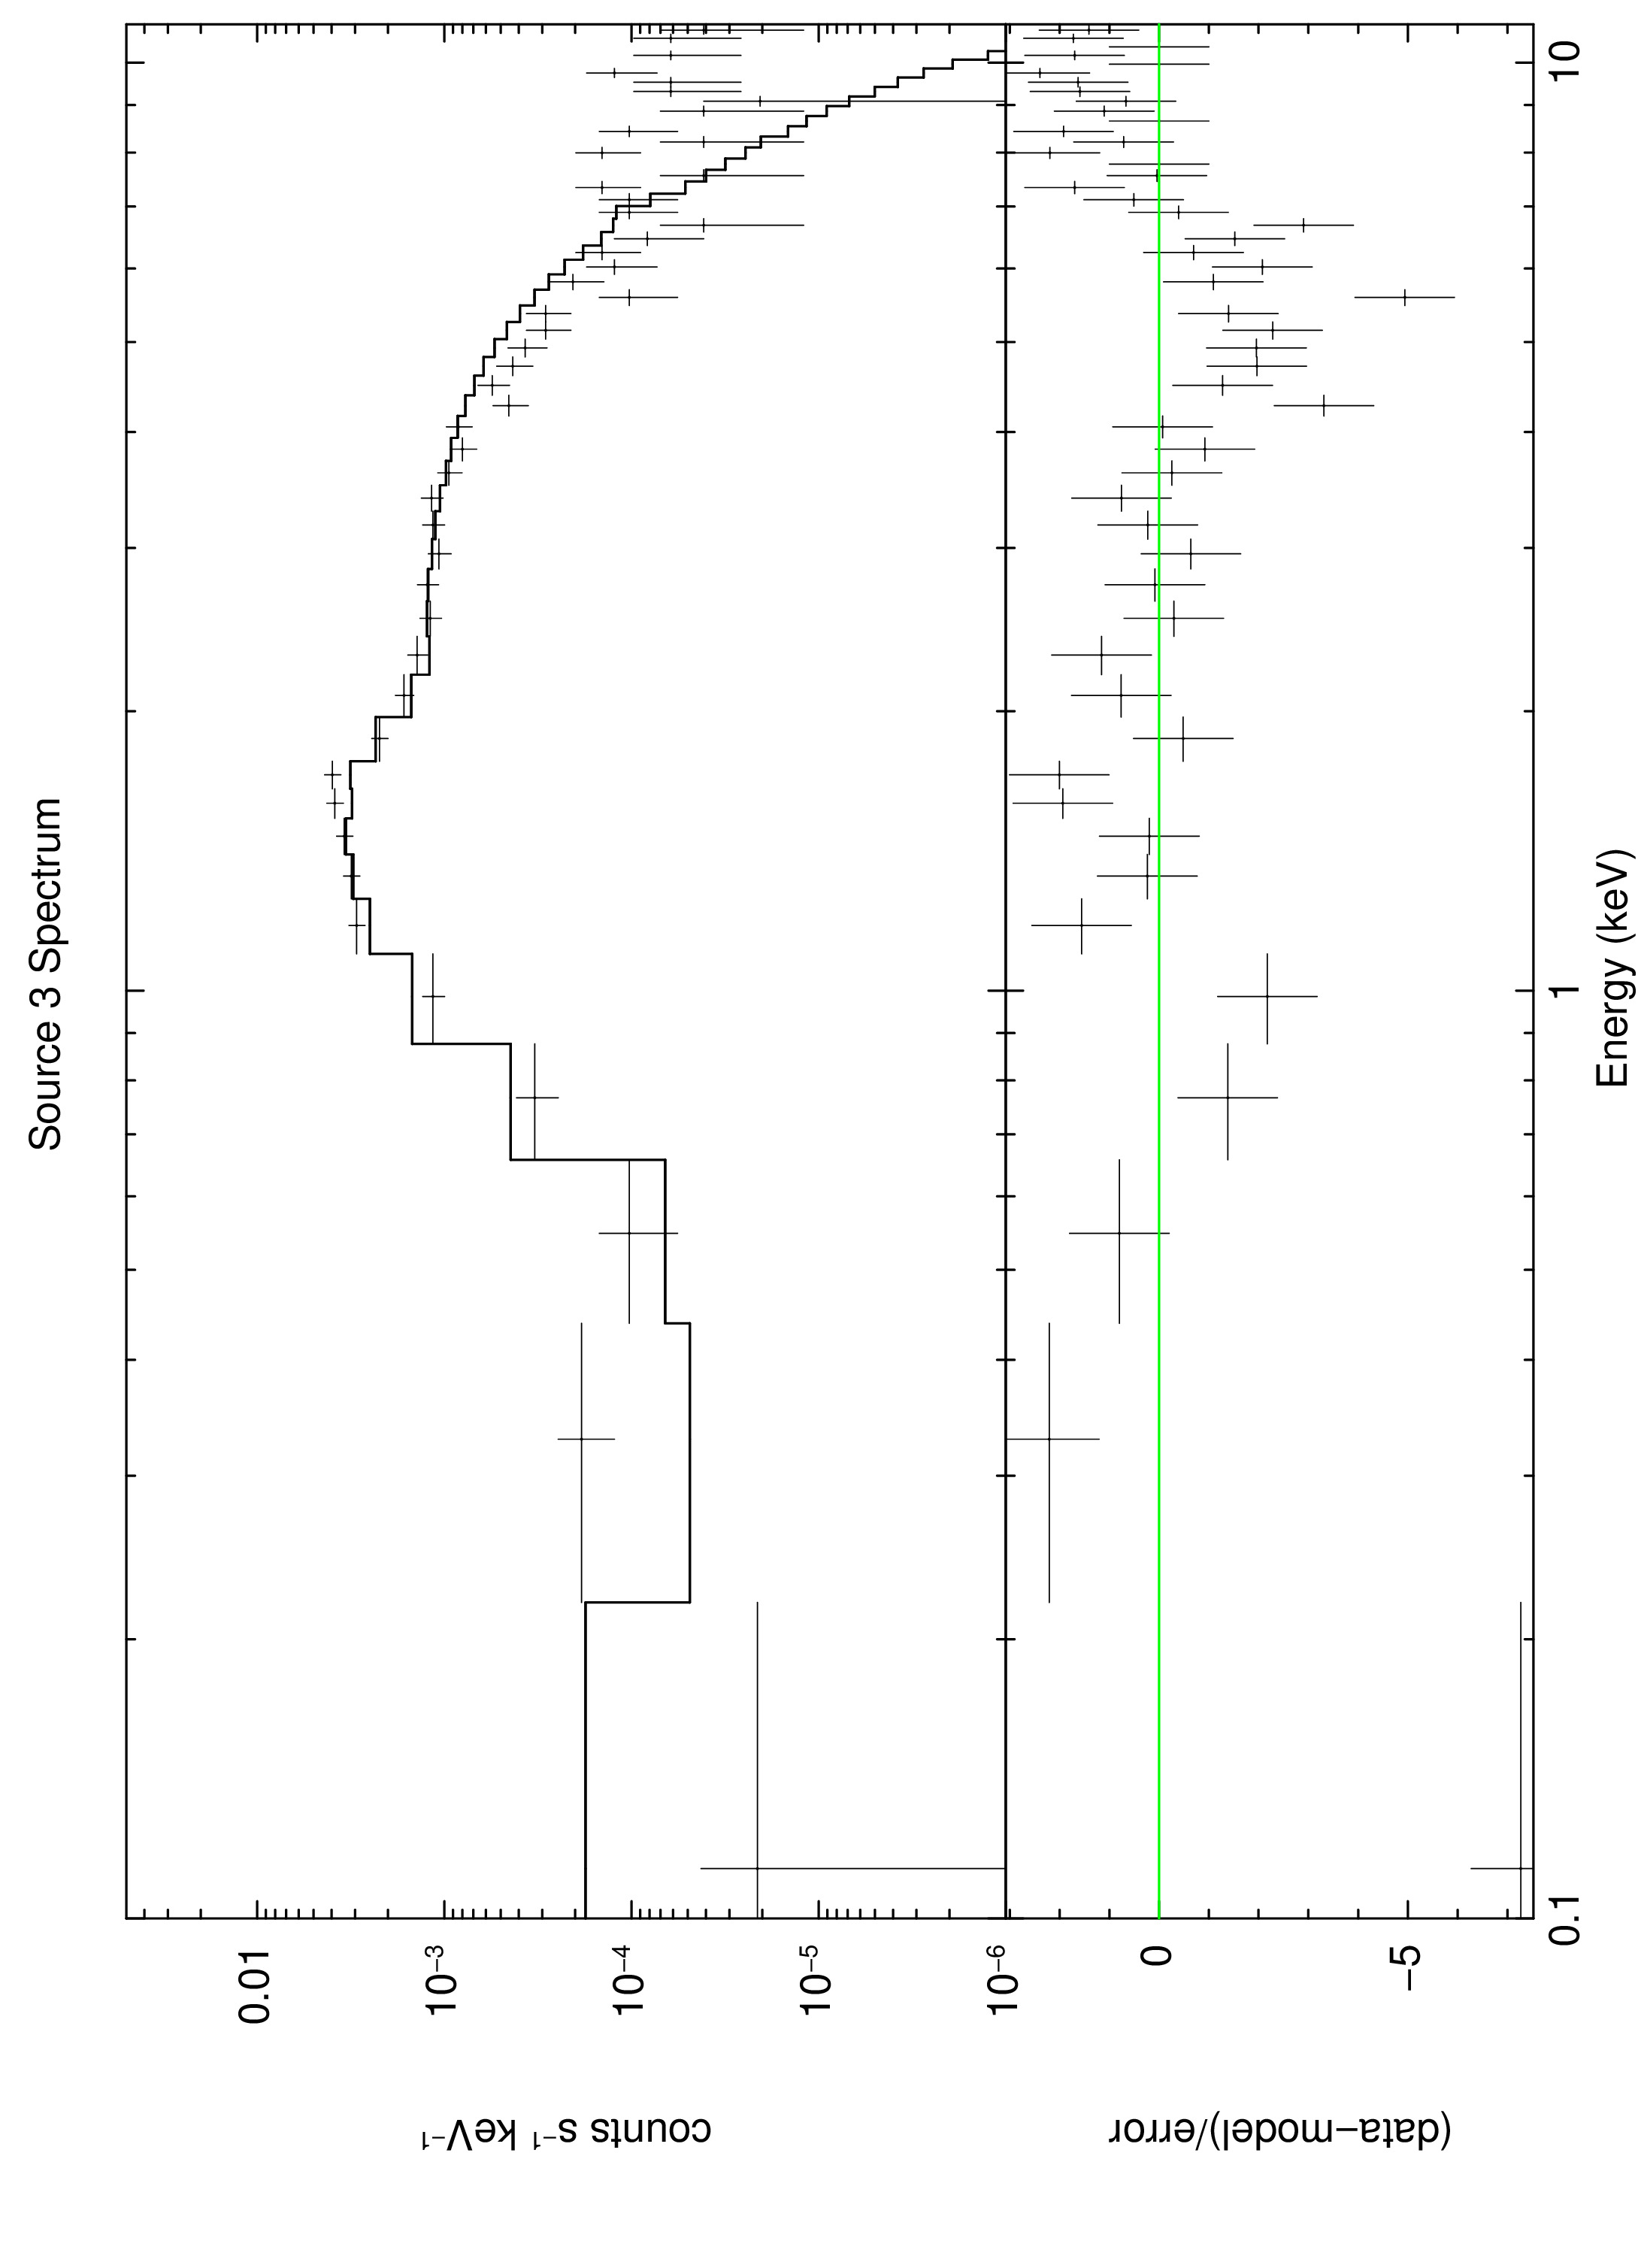
\includegraphics[angle=0, origin=c,width=.4\textwidth]{img/src-3-spectrum.jpg}}\qquad
    \subfloat[][]{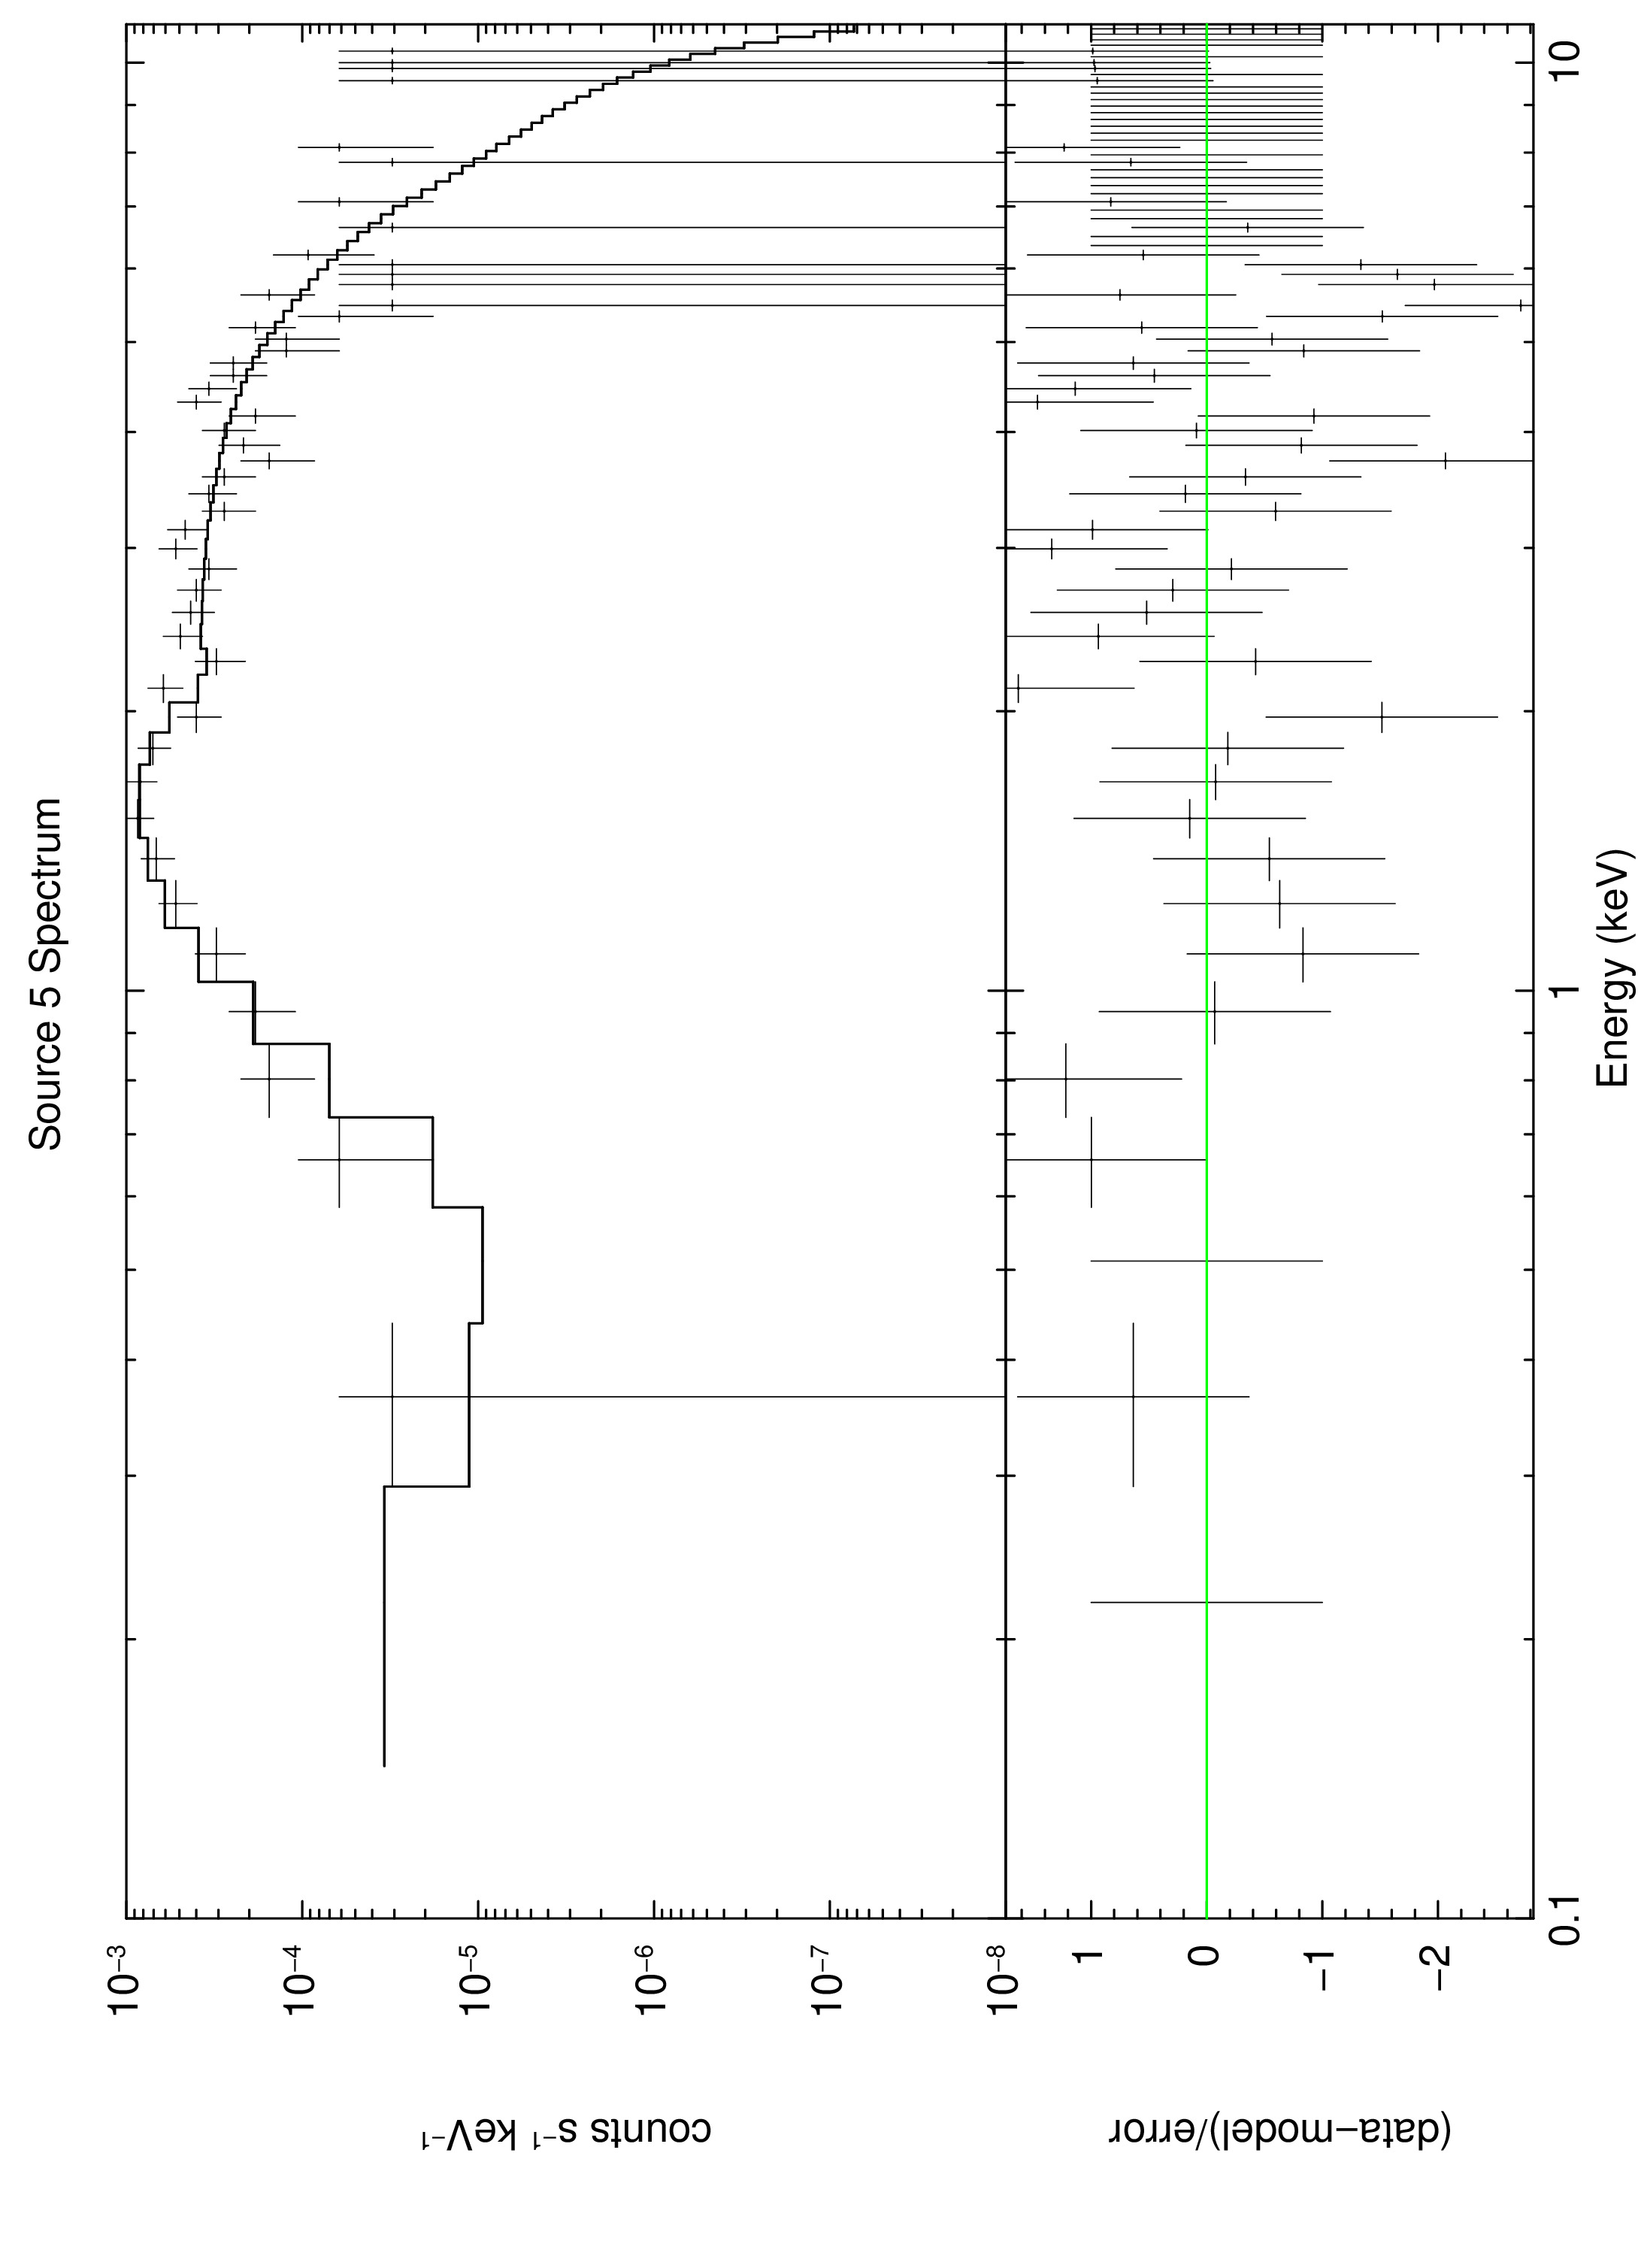
\includegraphics[angle=0, origin=c,width=.4\textwidth]{img/src-5-spectrum.jpg}}\\
    \subfloat[][]{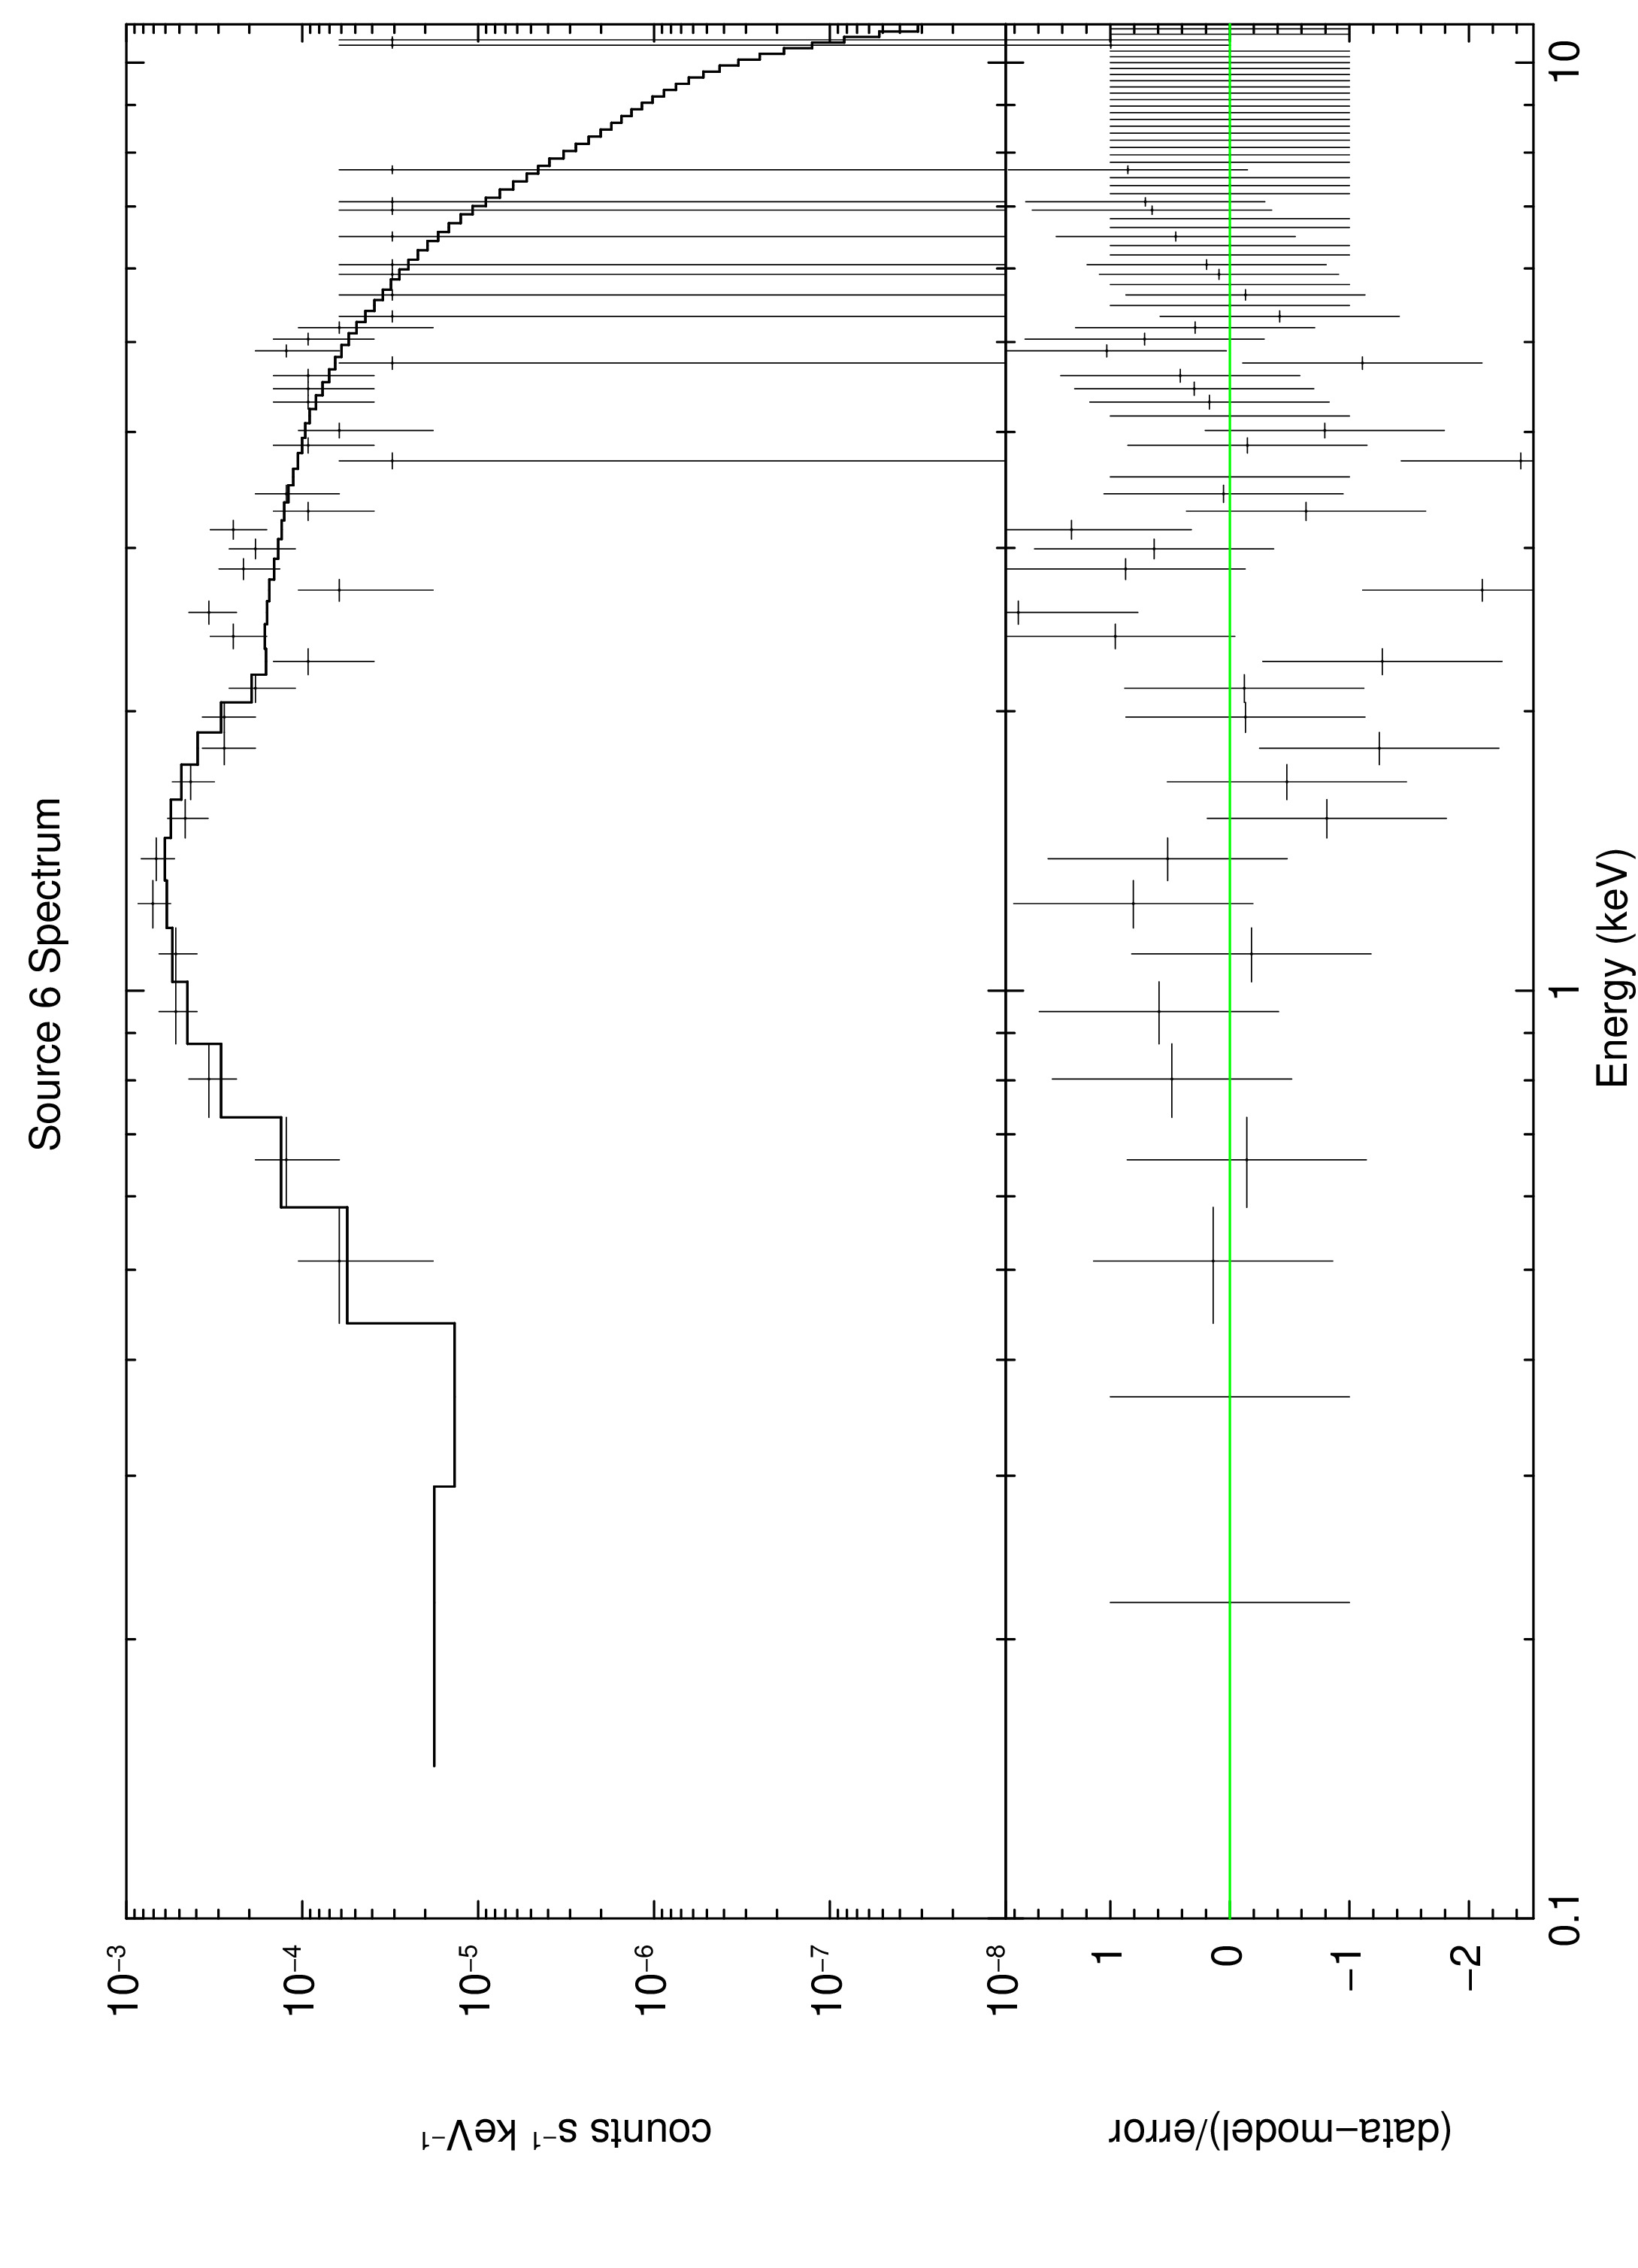
\includegraphics[angle=0, origin=c,width=.4\textwidth]{img/src-6-spectrum.jpg}}\qquad
    \subfloat[][]{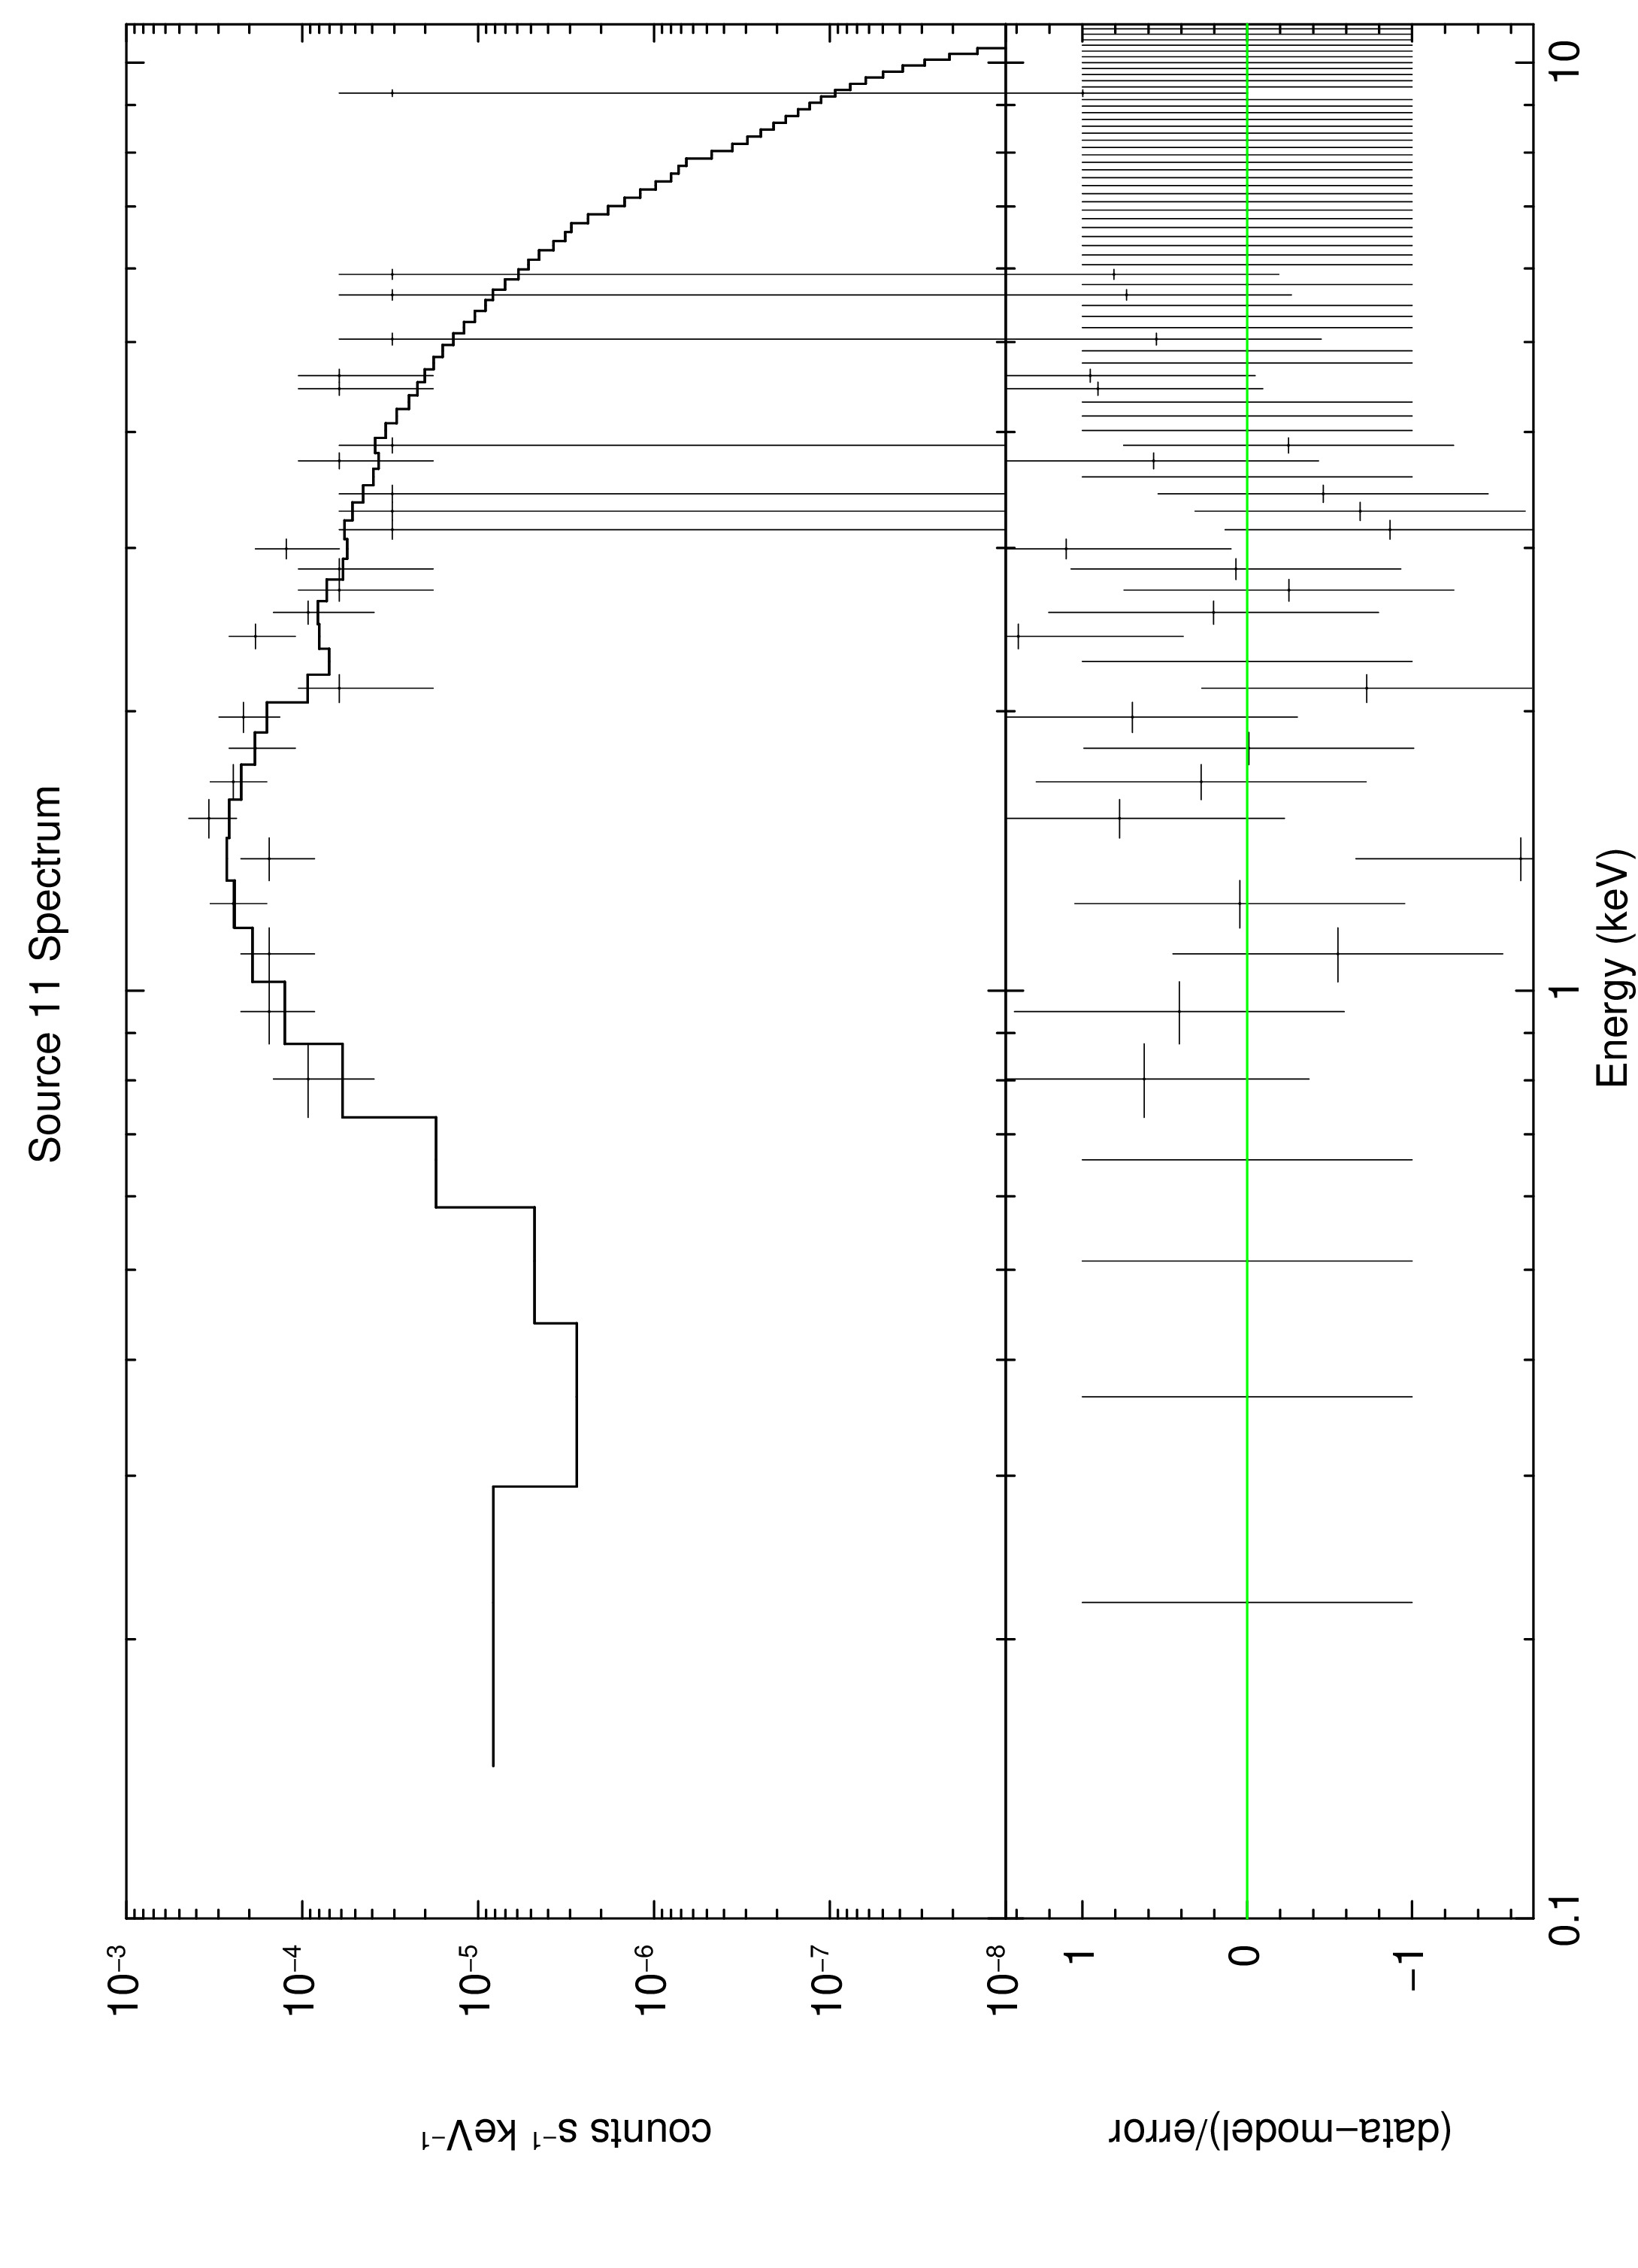
\includegraphics[angle=0, origin=c,width=.4\textwidth]{img/src-11-spectrum.jpg}}
    \caption{A selection of fitted spectra and residuals. {\bf (a)} is source 3, which is identified to be a CH star. {\bf (b)} is a cataclysmic variable with high internal absorption, with {\bf (c)} being an example of a CV with cluster average absorption. Finally {\bf (d)} is a RGB/SGB-a star. Note that the binning is performed for plotting only and is not present during fitting.}
    \label{fig:main-4-spectra}
\end{figure}

\subsection{Source 3: A CH star}
One of the more notable conclusions from Ref \cite{Henleywillis2018} is that the source 3, previously identified optically as a CH star, may be a symbiotic binary, the first such star in a globular cluster. In this analysis, the expected higher than cluster medium absorption ($n_H\approx4\times10^{21}\text{cm}^{-2}$) was replicated in the modelling. However a much higher plasma temperature ($kT\approx25\text{keV}$) was observed in the fitting. With that being said, these values still fall within a reasonable range for what a symbiotic binary would be expected to have \cite{Luna2013}. To confirm this conclusion further observations would need to be made, however. For one, we expect the hard x-ray emission to time-variable, not only this, but symbiotic stars with high energy emissions ($kT\sim$5-50keV) experience the greatest variability in their UV spectrum\cite{Luna2013}. 

\subsection{Source 5 and 6: Cataclysmic variables}
There are many CVs identified within the globular cluster. Of the 13 brightest sources listed here, 9 of them have been identified as CVs. Interestingly, though 6 of these CVs required higher than cluster average absorption to be fitted correctly (just as in Ref \cite{Henleywillis2018}). In the original paper, two explanations are given for this. Firstly, if the CV's are orientated such that the binary system is eclipsed, then high absorption is known to occur \cite{Heinke2005}. It is very improbable that this explain all of the high $n_H$ CVs present within this observation, simply due the statistical improbability of having so may systems orientation in such a specific manner. Instead, \cite{Henleywillis2018} suggest that the high absorption could be due to magnetism being present within some of the systems. These are CV systems with 'mid-strength' magnetic field, strong enough to disrupt the accretion somewhat, but not stall it entirely. It is estimated, though, that magnetic CVs only make up around 20\% of all CVs, so this does not directly explain the large proportion of high $n_H$ CVs present in this source list. However, also due to the magnetic field direct accretion flow close to radially, it is expected the magnetic CVs will exhibit a brighter x-ray emission then non-magnetic CVs \cite{Pretorius2013}. This bias in the sampling of the source list could go a long way in explaining the large fraction of high $n_H$ CVs present. Though ultimately, again, more observations will be required to confirm this explanation, potentially performing spectral fitting of a larger population of CVs with $\omega$ Cen will reveal the true proportion of the high $n_H$ CVs present.

\section{Conclusion}
An analysis of {\it Chandra} ACIS-I observations of the globular cluster $\omega$ Cen has been replicated. Two datasets were merged an utilised, to give a total exposure time of ~220ks, allowing good detection of faint sources. The 13 brightest sources were selected and identified within the results of the original study. A spectral fitting of these sources was performed, modelling them with a composite model within {\sc xspec}, {\sc tbabs} and {\sc vmekal}, providing insight into the internal absorption and temperature of the sources identified. For the most part, the fitting parameters are within the 90\% confidence interval given, and so match the original analysis. For the parameters that vary greatly (eg. some temperature values), it was shown that likely they are due to local minima in the fitting process, and thus may be disregarded. The CH star, which is source 3, had similar parameters to that described originally, though with a lower $n_H$ and higher $kT$. Thus, leading a similar identification of this system being a possible symbiotic star. Also replicated, was the large proportion of high $n_H$ CVs present in the source list. This again lends further credence to the explanation given in the original paper. Overall, this replication report strongly supports these conclusions given in the study, however, with all things, further observations are required to validate these claims, namely observations within different energy bands, such as UV, and spectral fitting of fainter CVs. 

\nocite{*}
\bibliographystyle{plain}
\bibliography{references}
\newpage

\appendix
\section{Spectra for all sources identified}
\begin{figure}[H]
    \centering
    \subfloat[][]{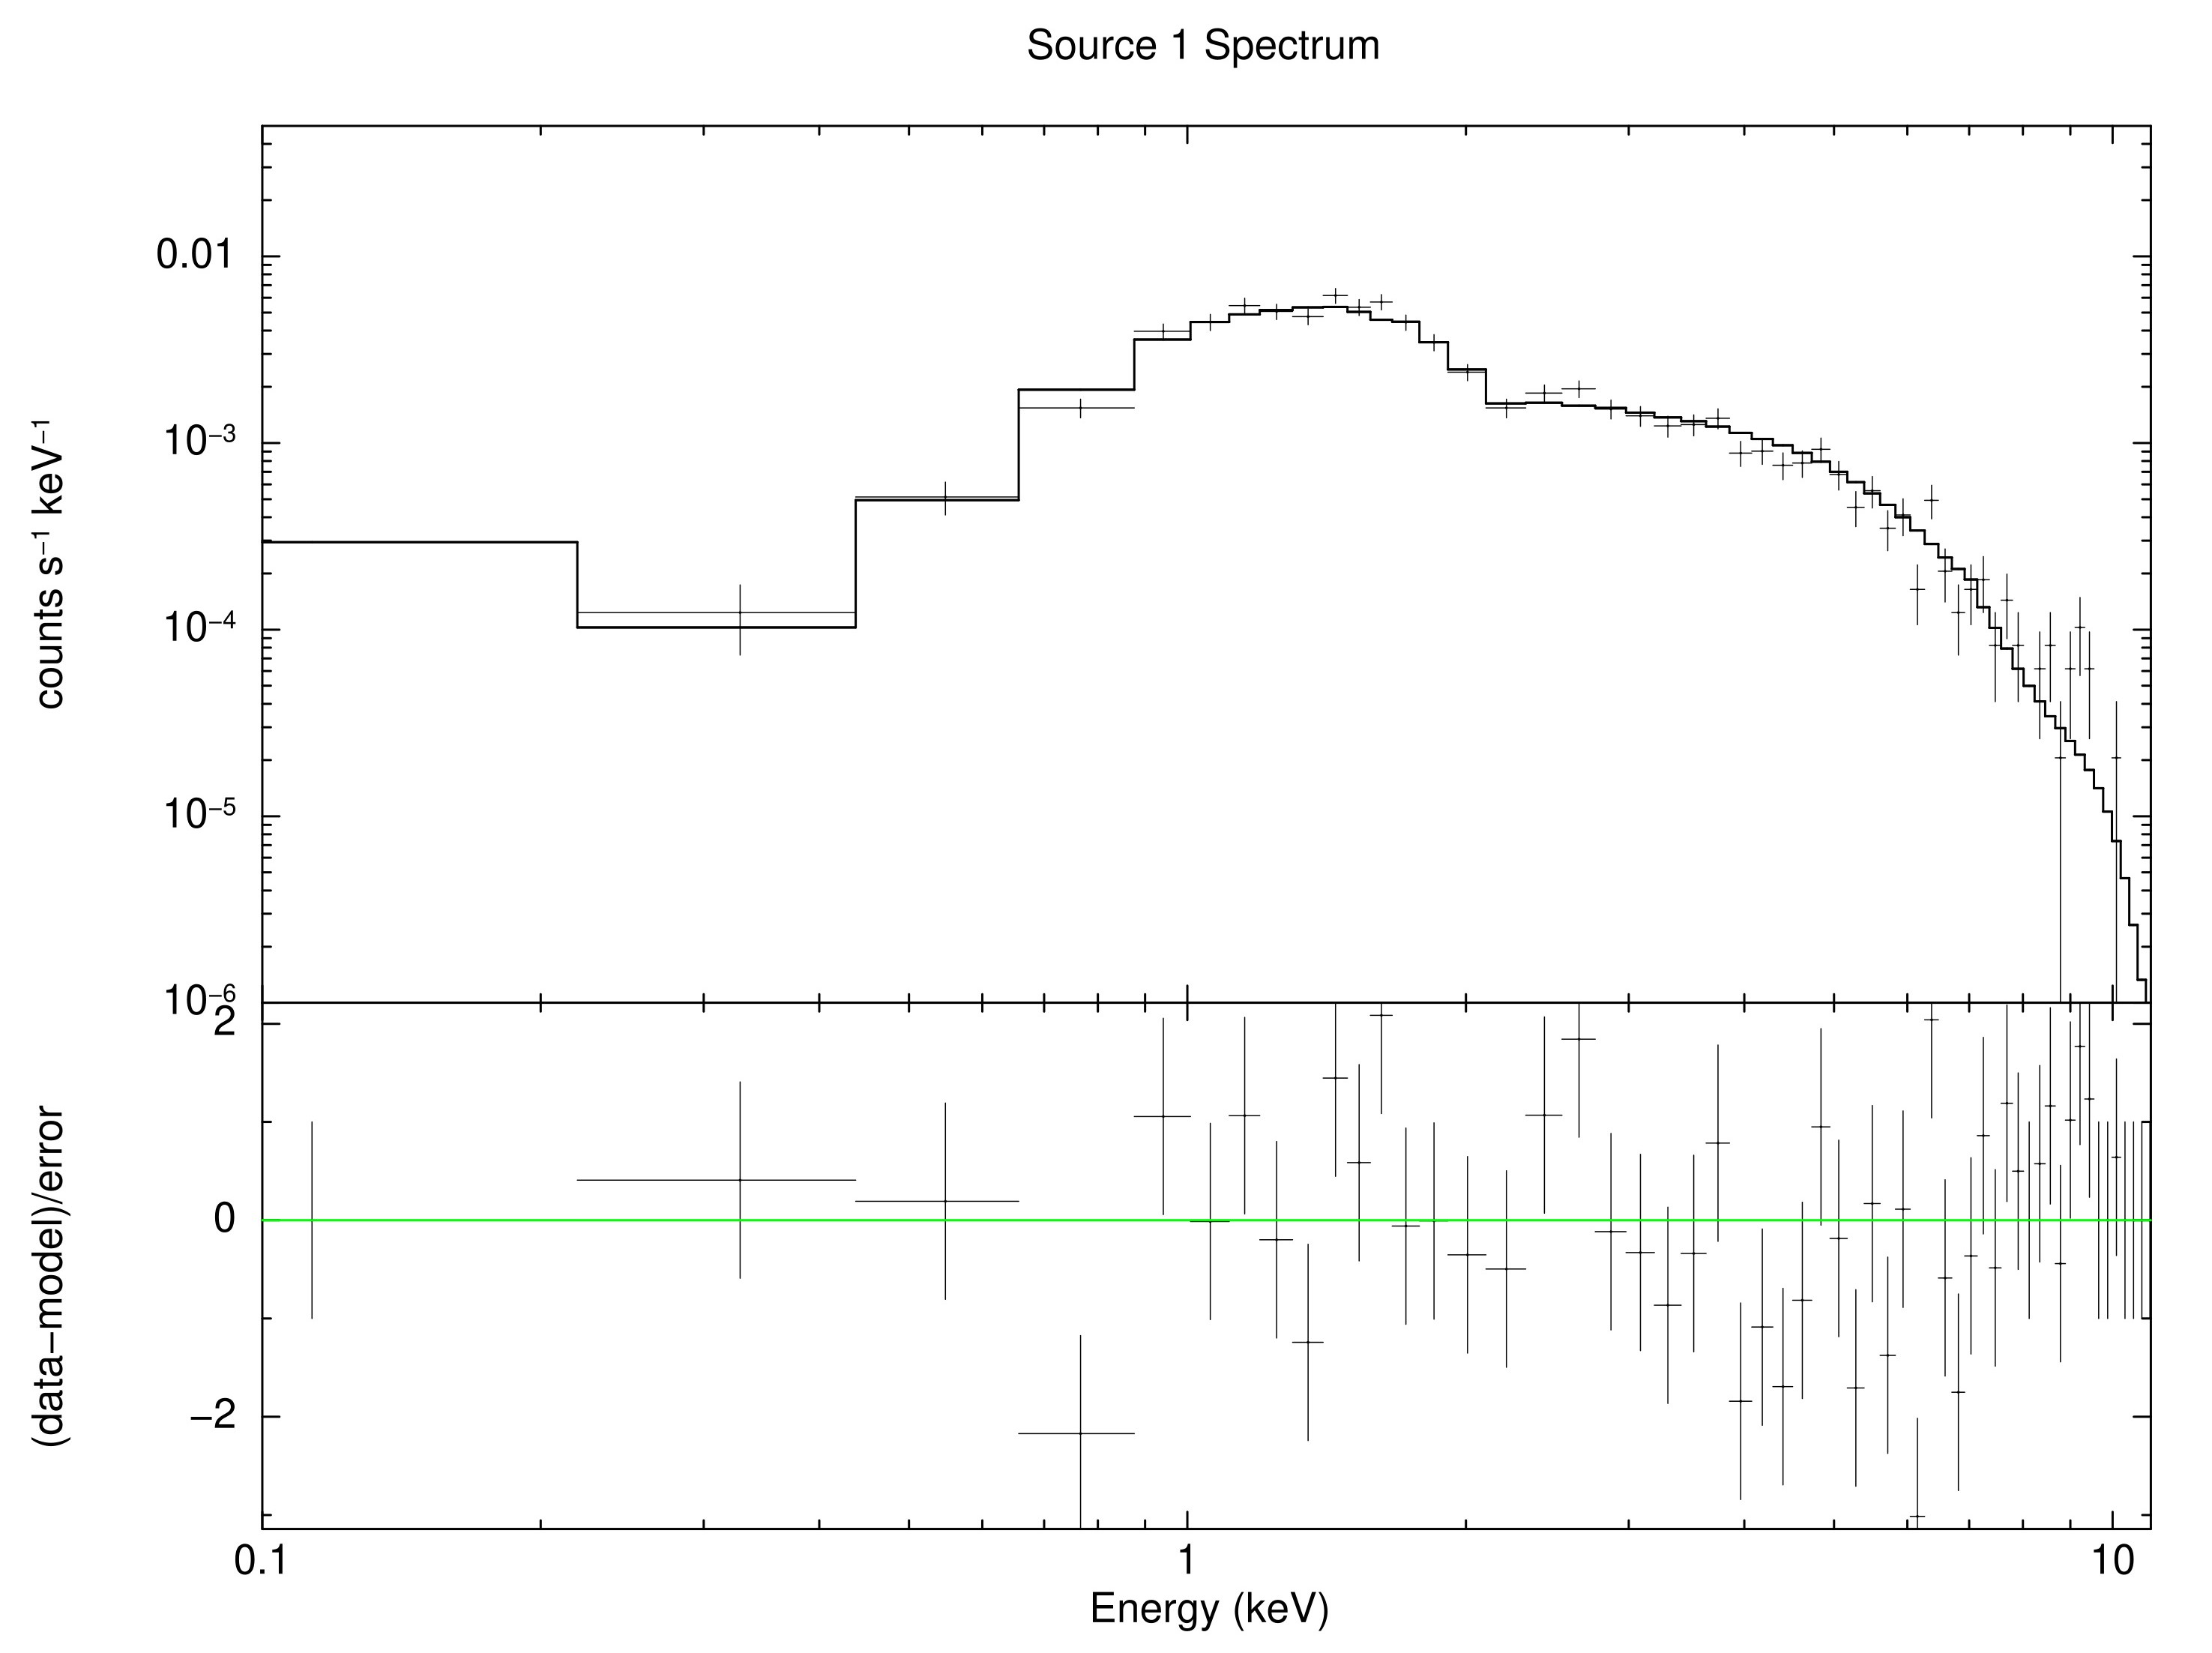
\includegraphics[angle=90, origin=c,width=.45\textwidth]{img/src-1-spectrum.jpg}}\qquad
    \subfloat[][]{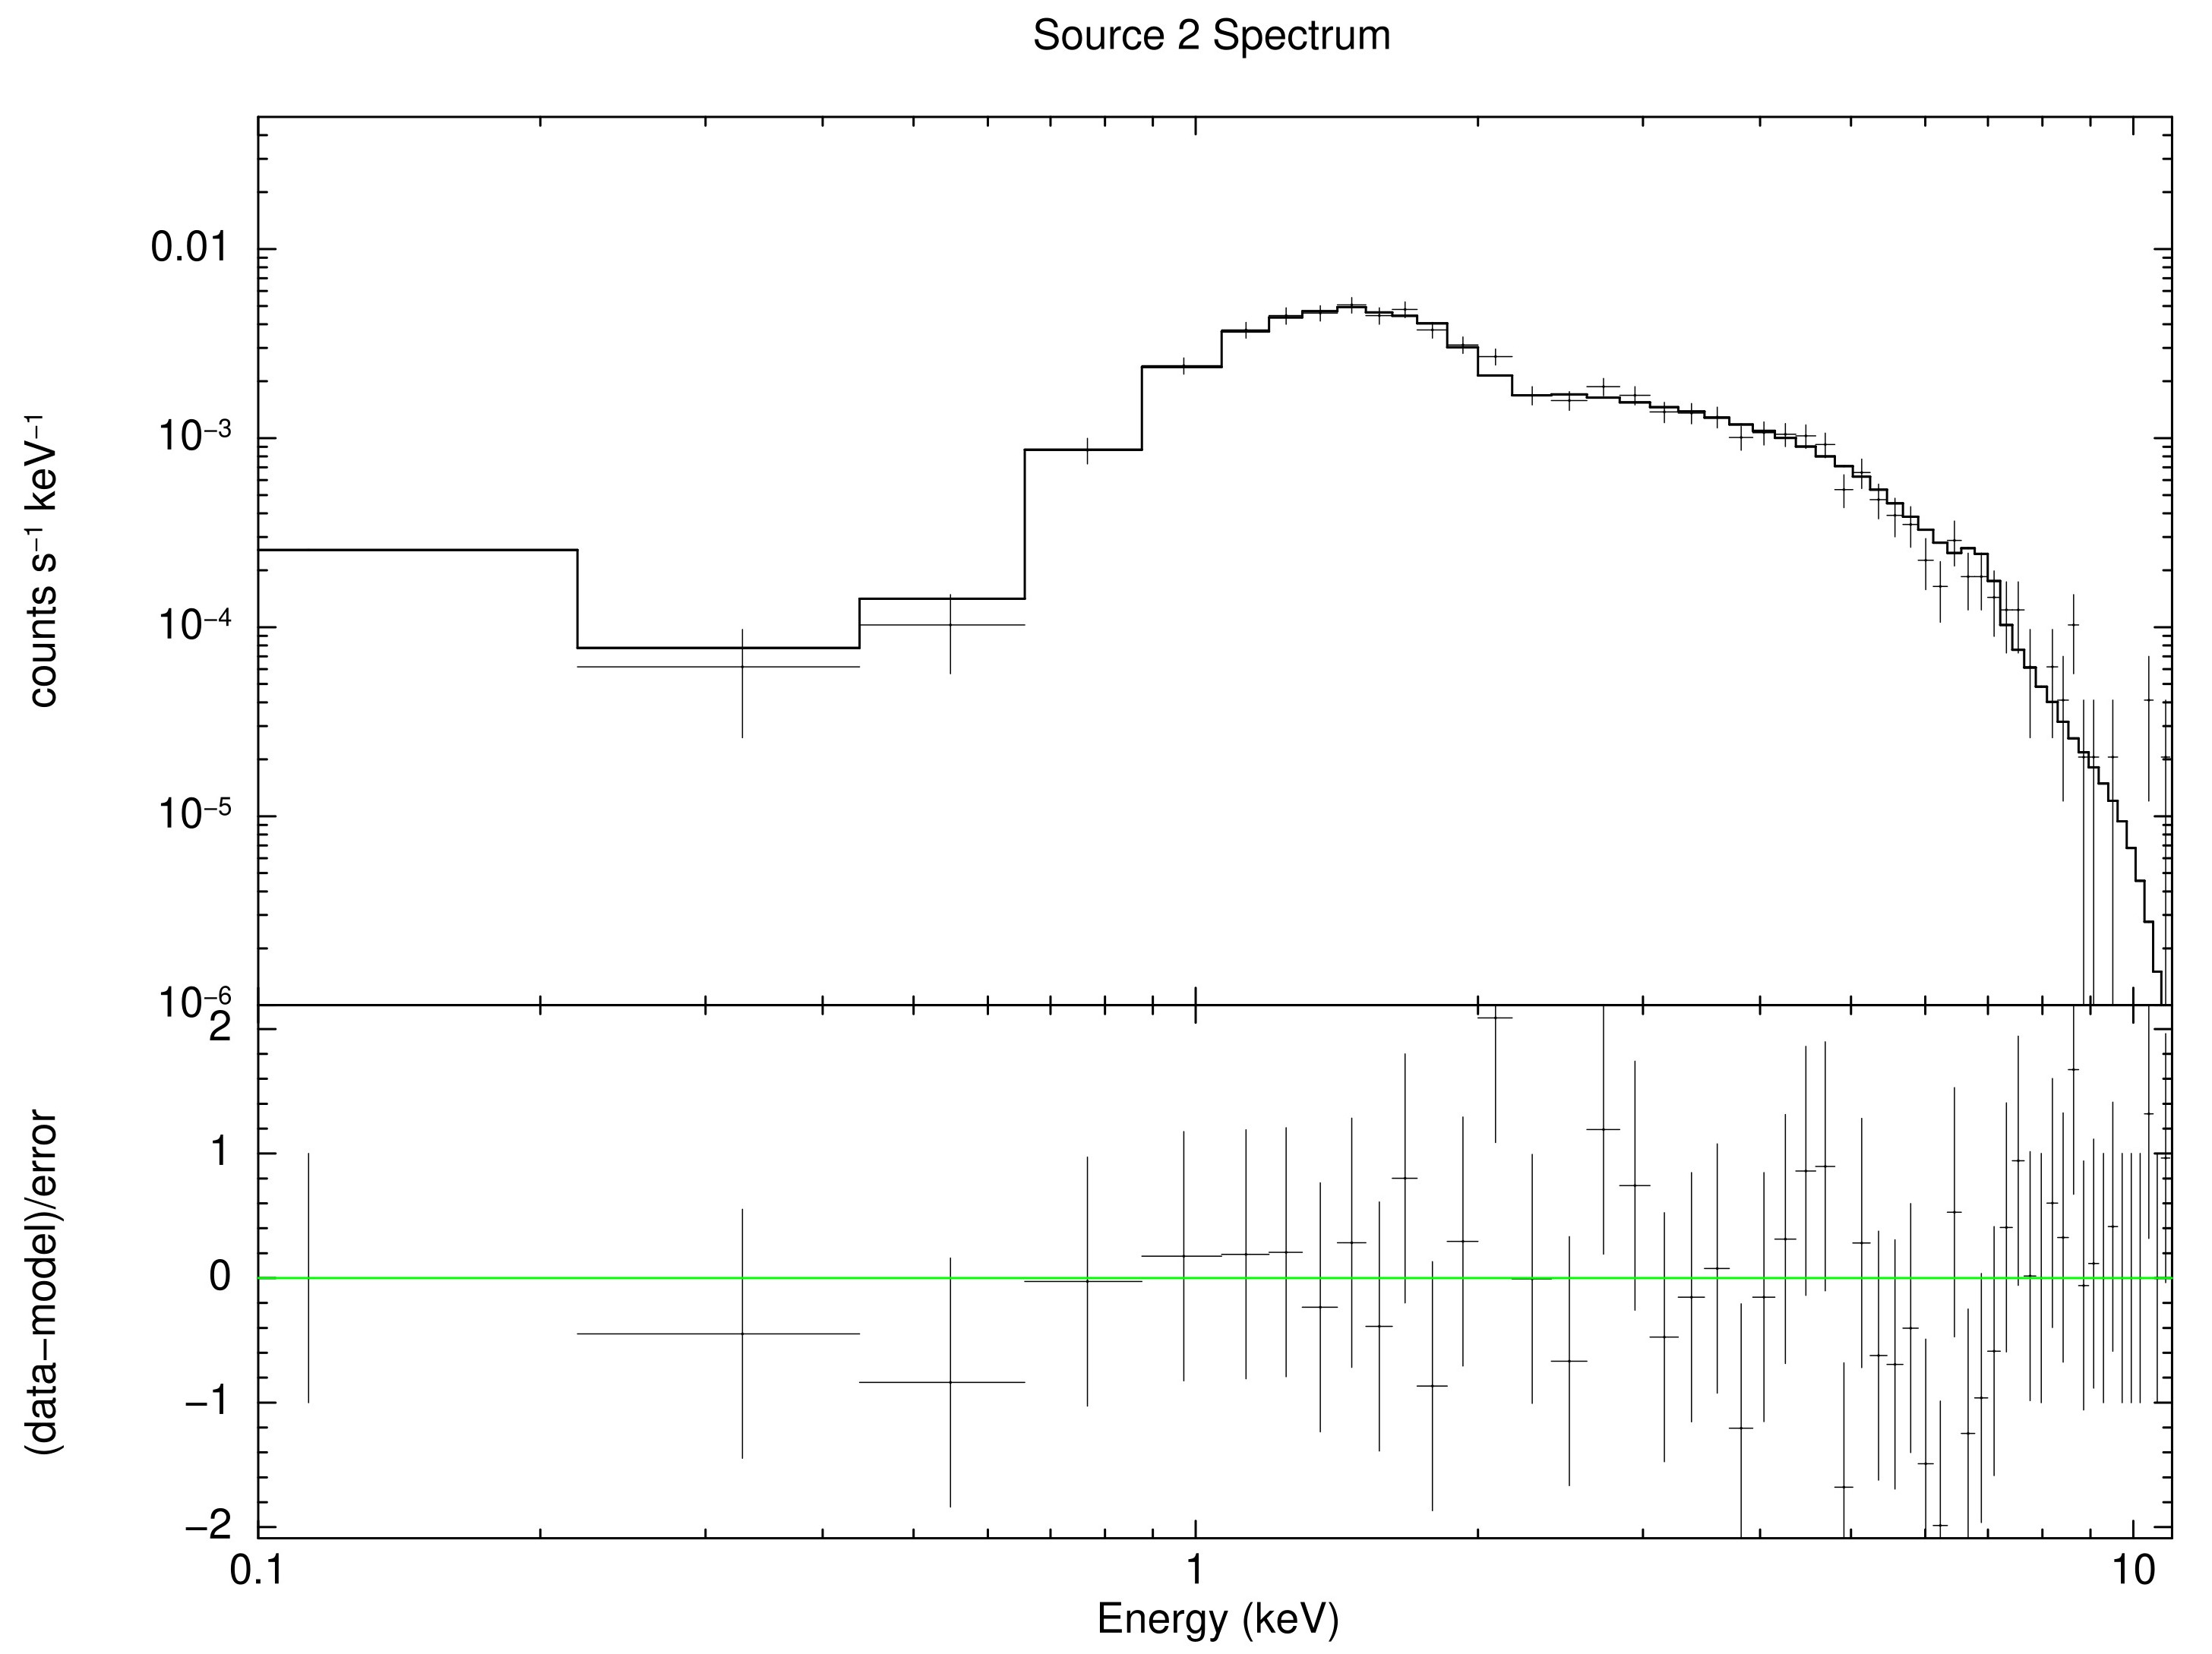
\includegraphics[angle=90, origin=c,width=.45\textwidth]{img/src-2-spectrum.jpg}}\\
    \subfloat[][]{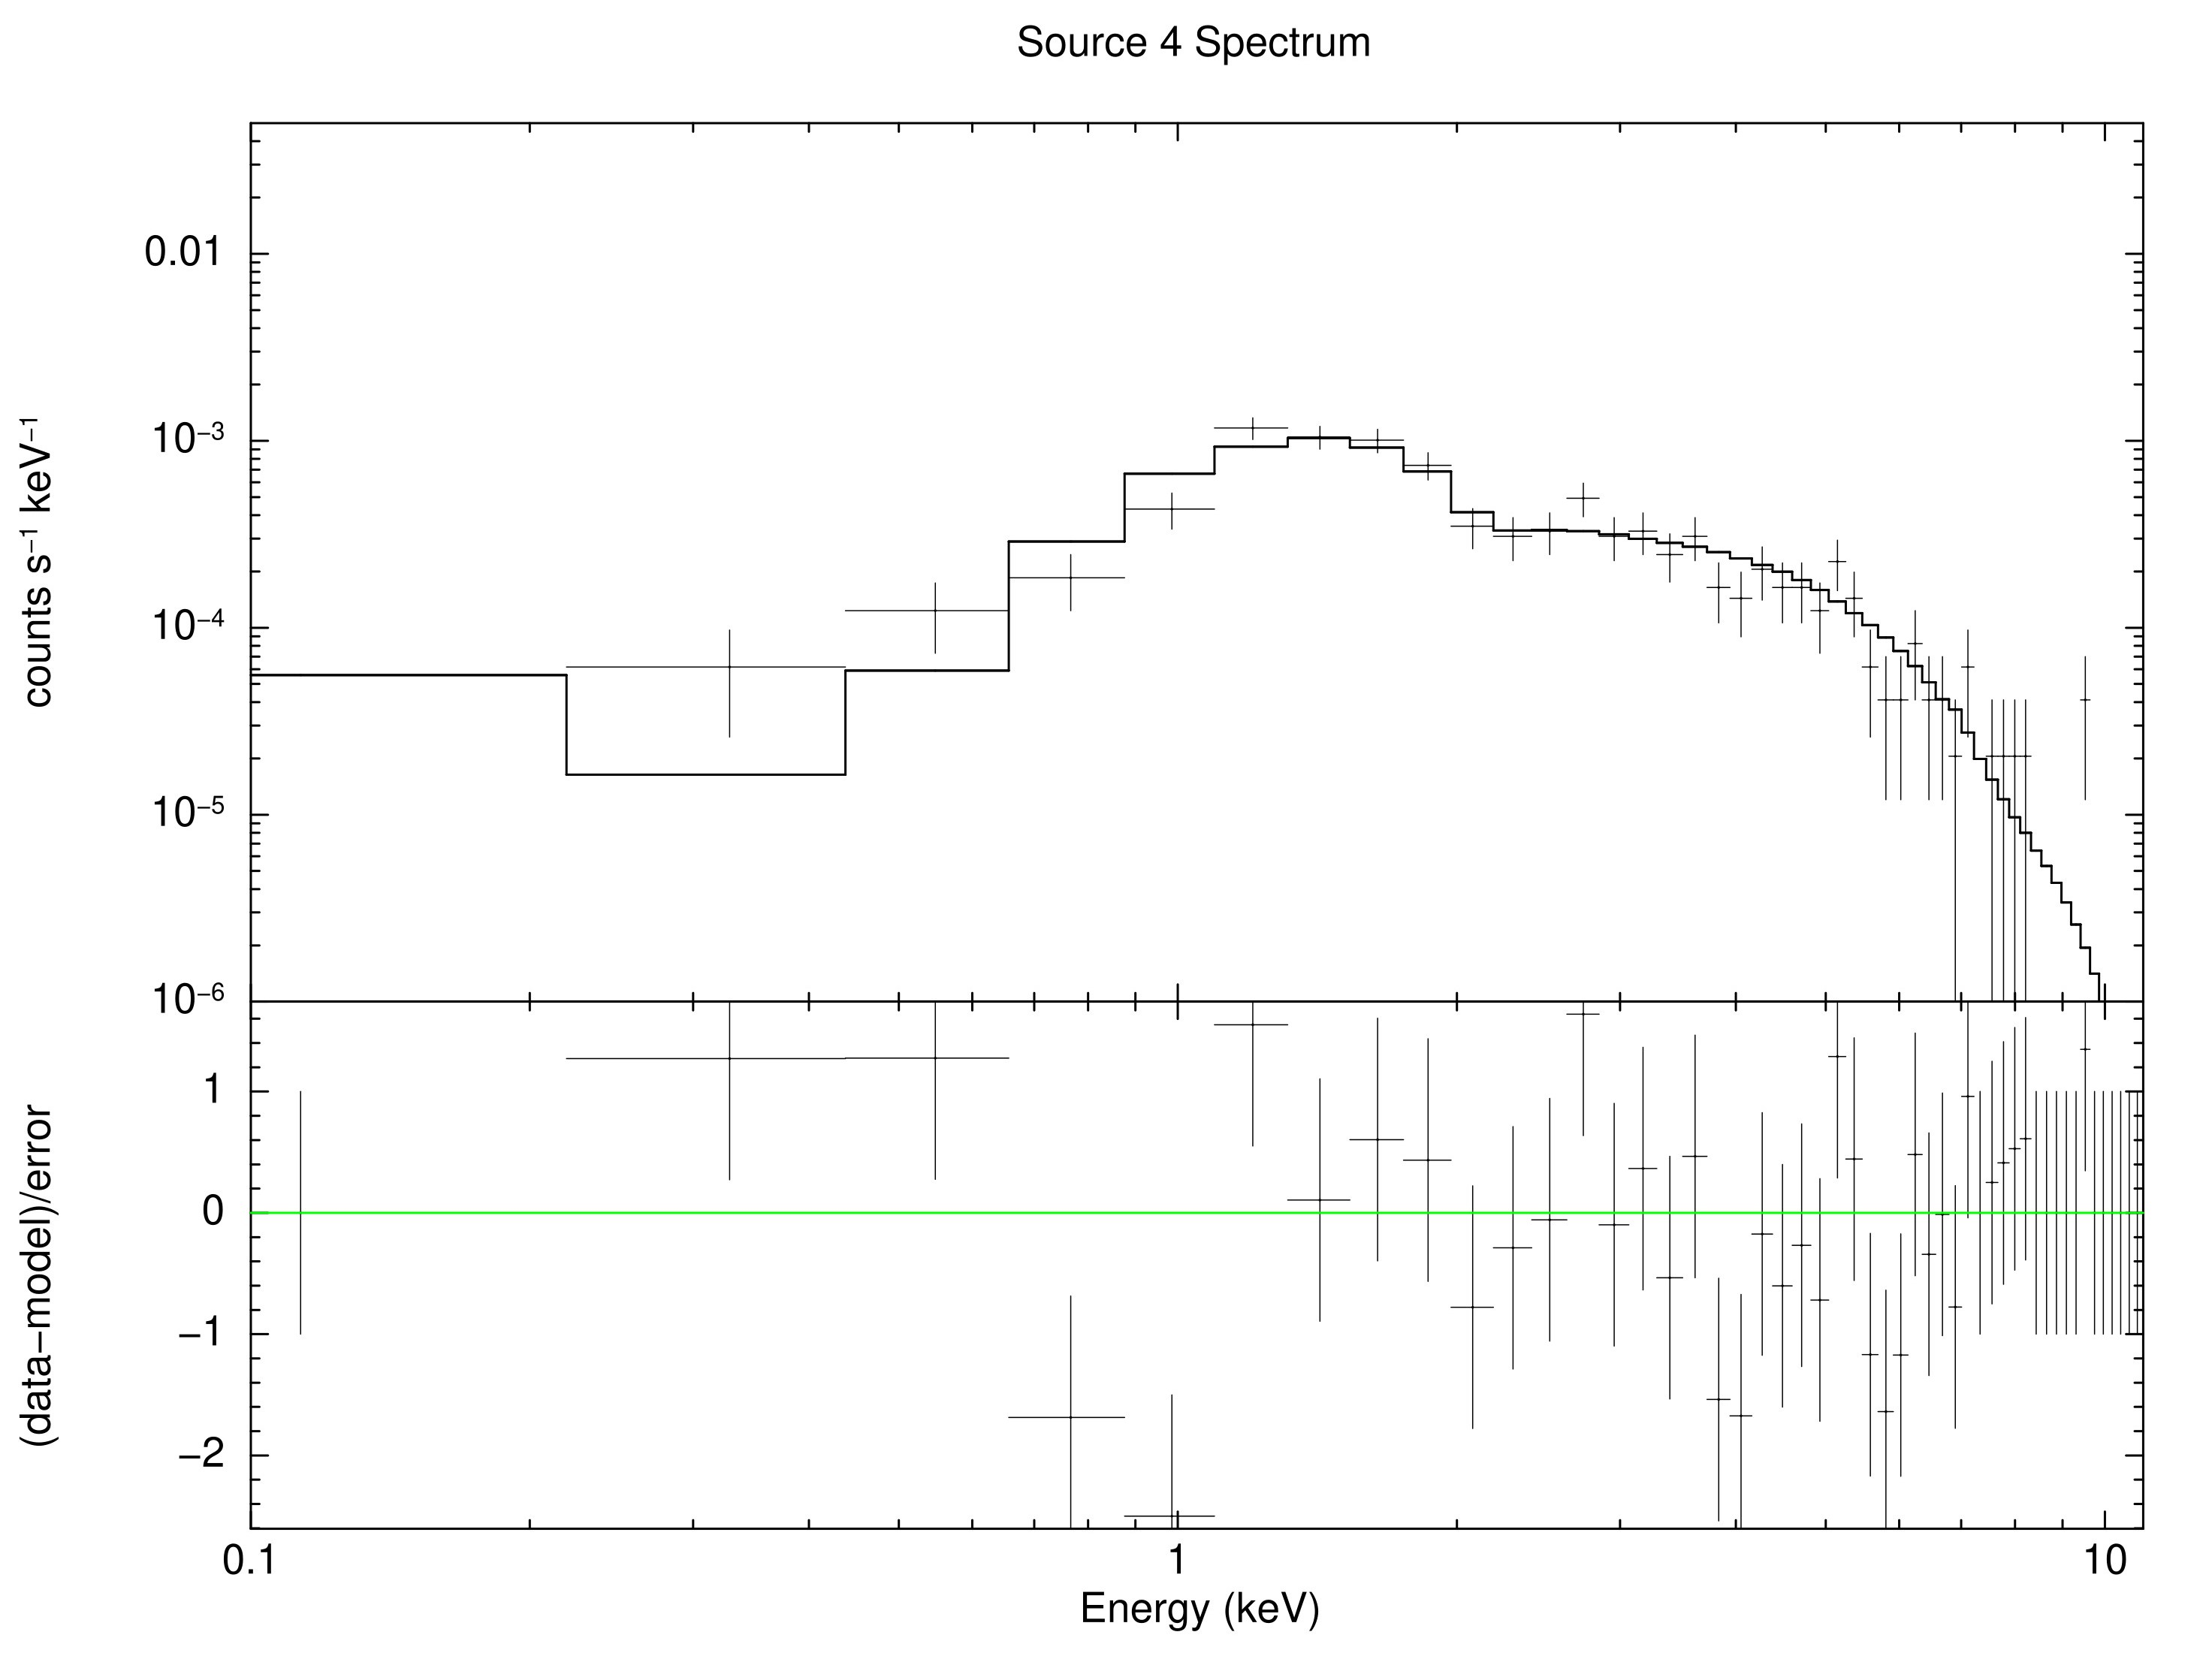
\includegraphics[angle=90, origin=c,width=.45\textwidth]{img/src-4-spectrum.jpg}}\qquad
    \subfloat[][]{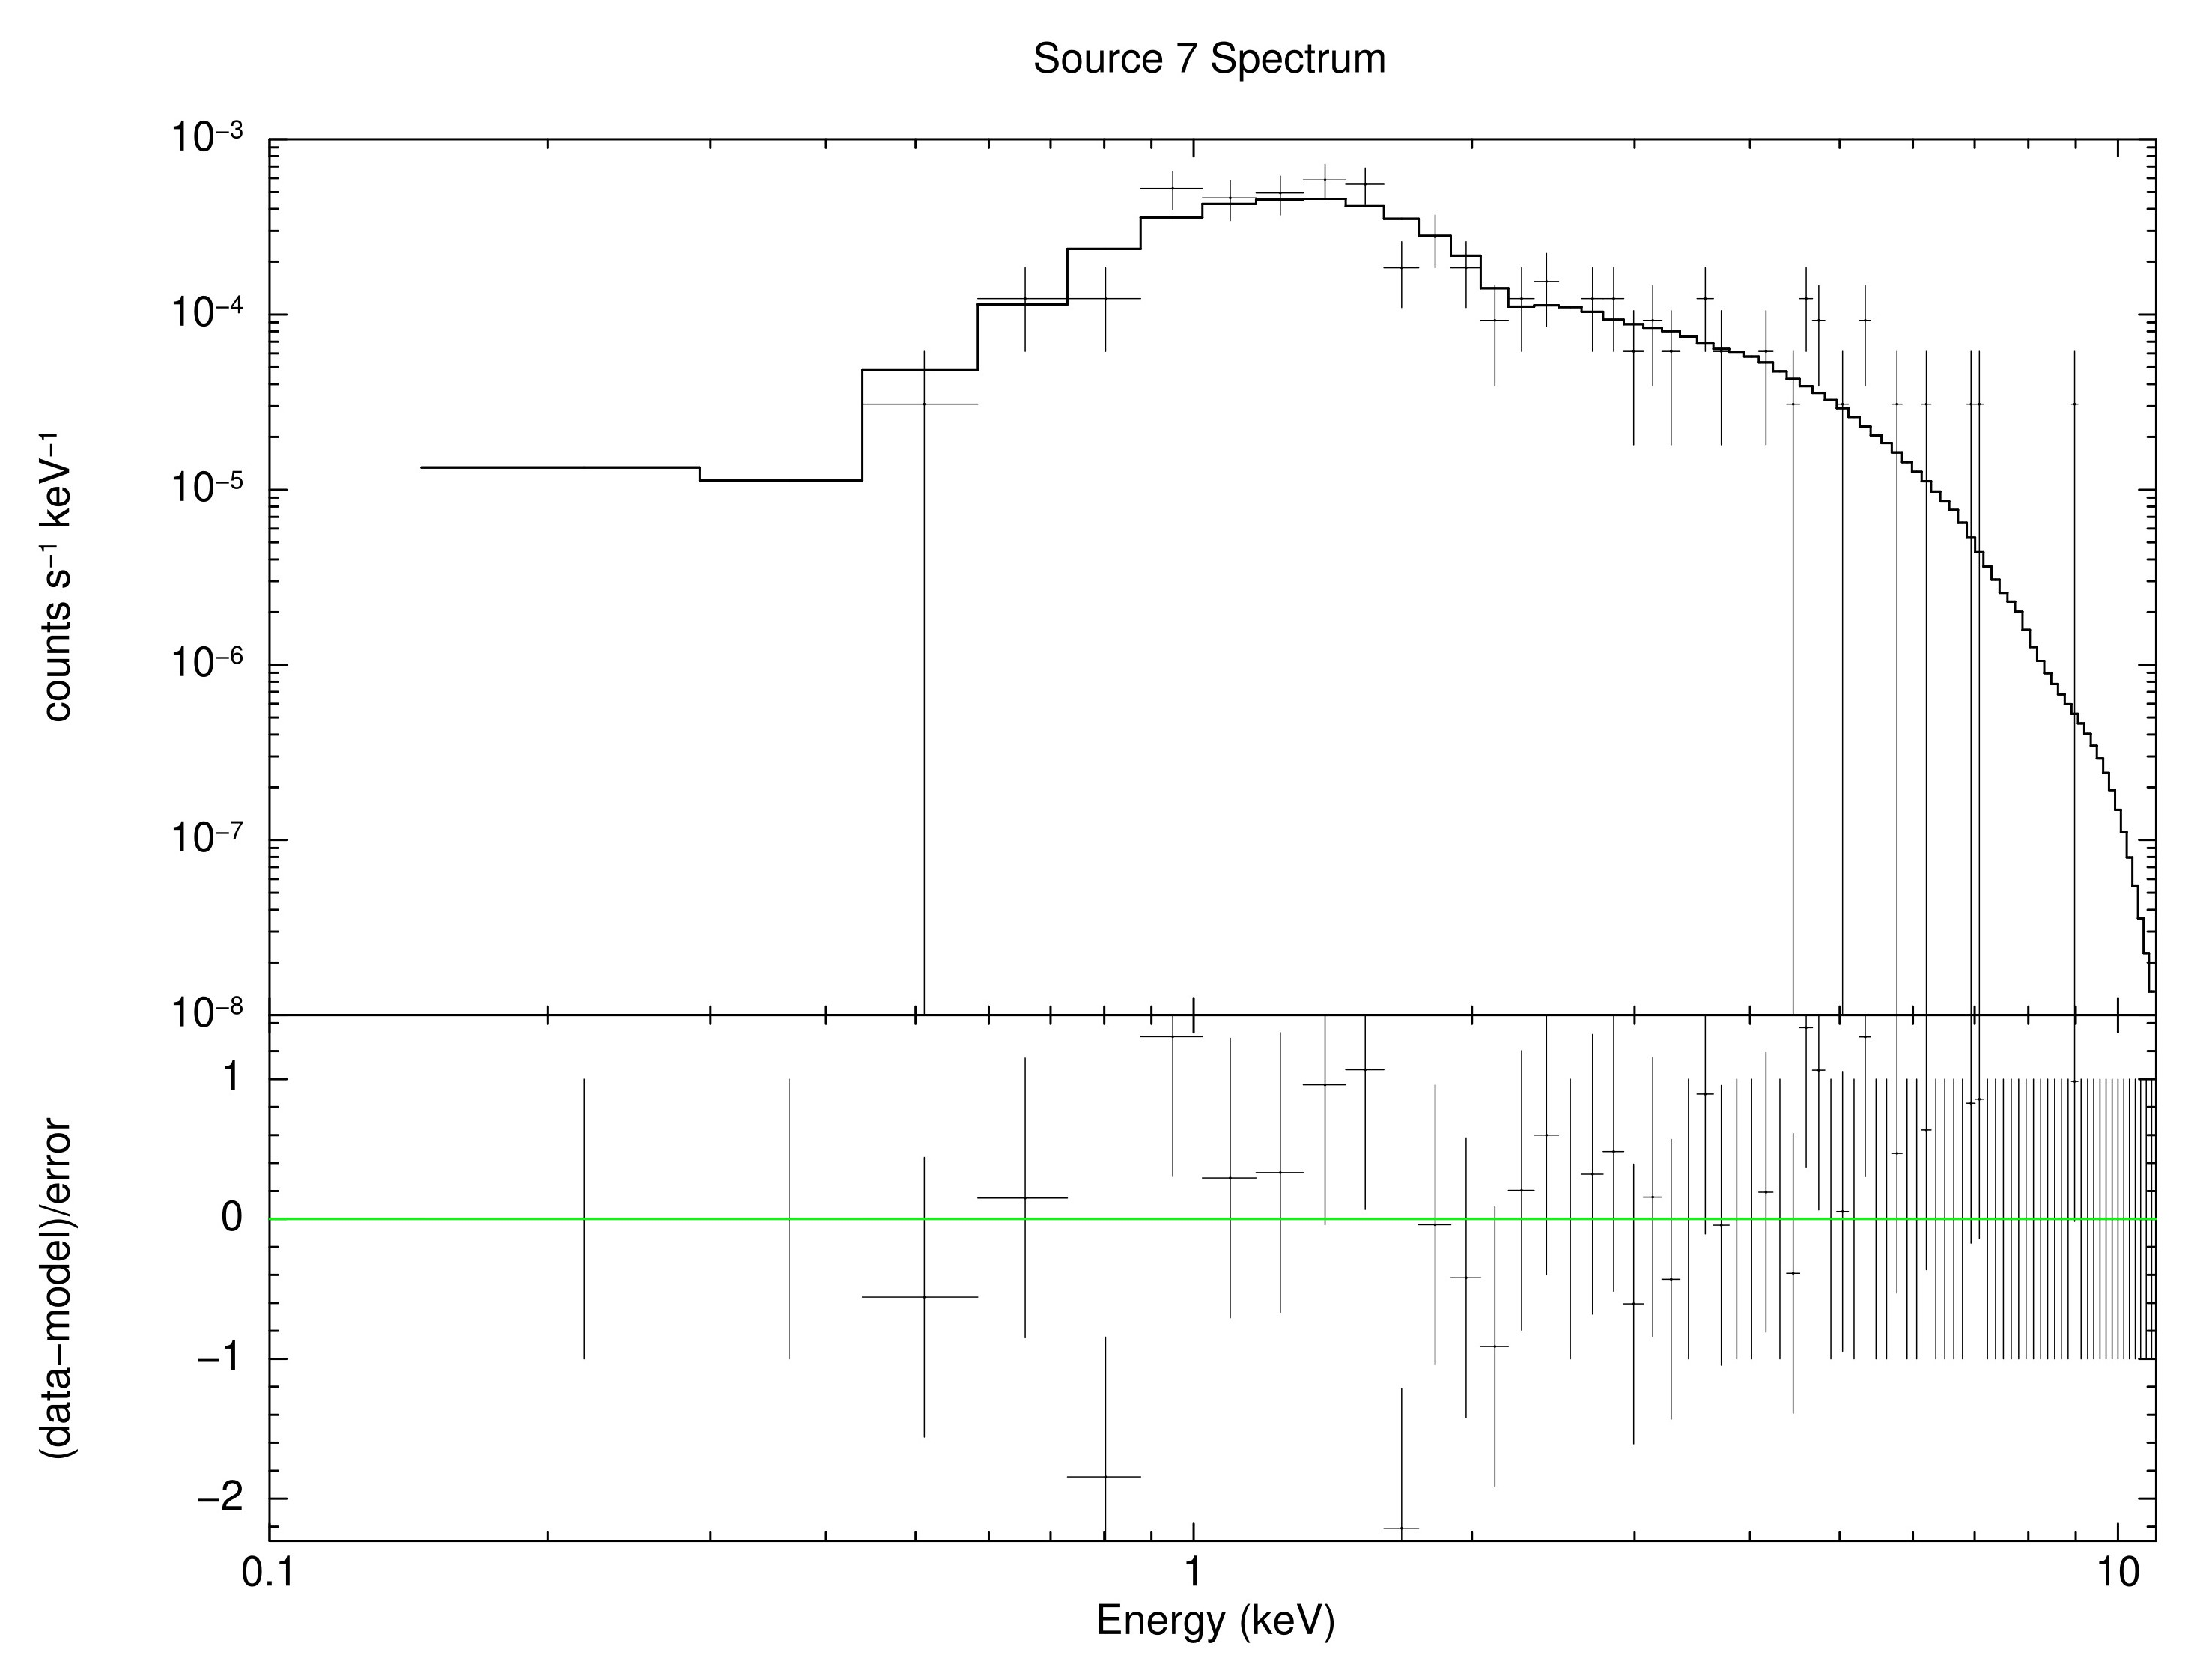
\includegraphics[angle=90, origin=c,width=.45\textwidth]{img/src-7-spectrum.jpg}}
    \caption{}
\end{figure}
\begin{figure}[H]
    \centering
    \subfloat[][]{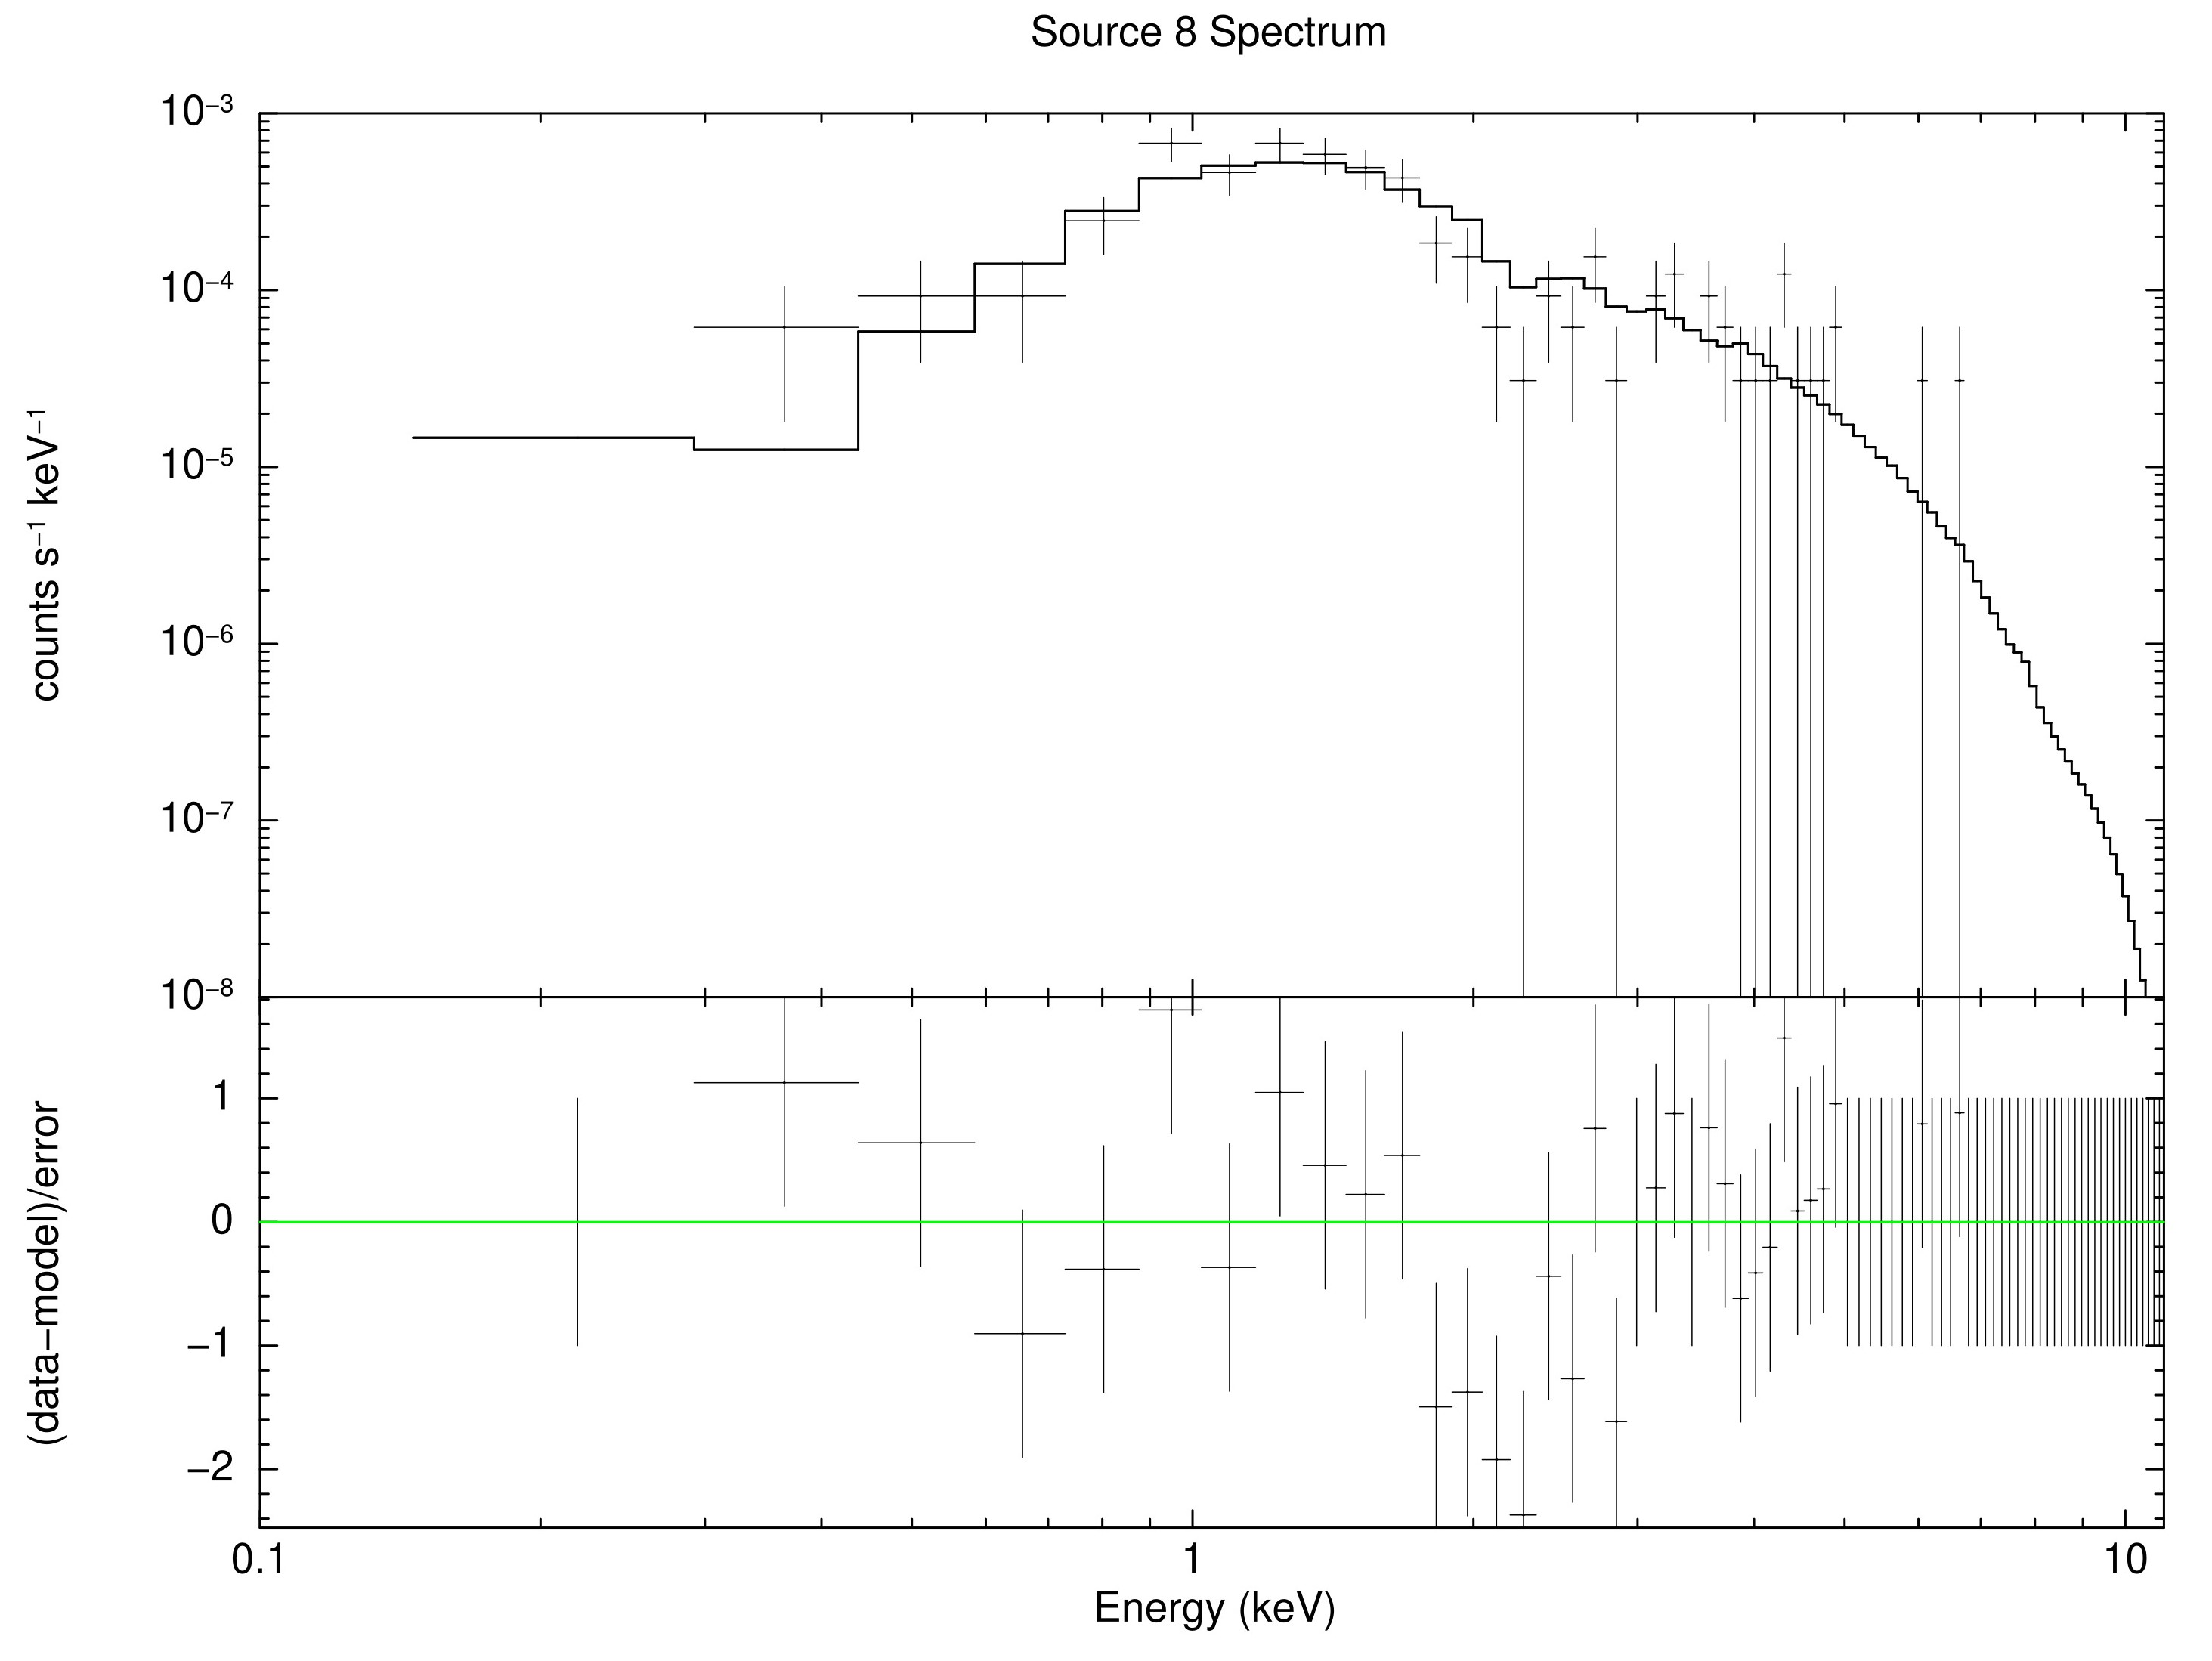
\includegraphics[angle=90, origin=c,width=.45\textwidth]{img/src-8-spectrum.jpg}}\qquad
    \subfloat[][]{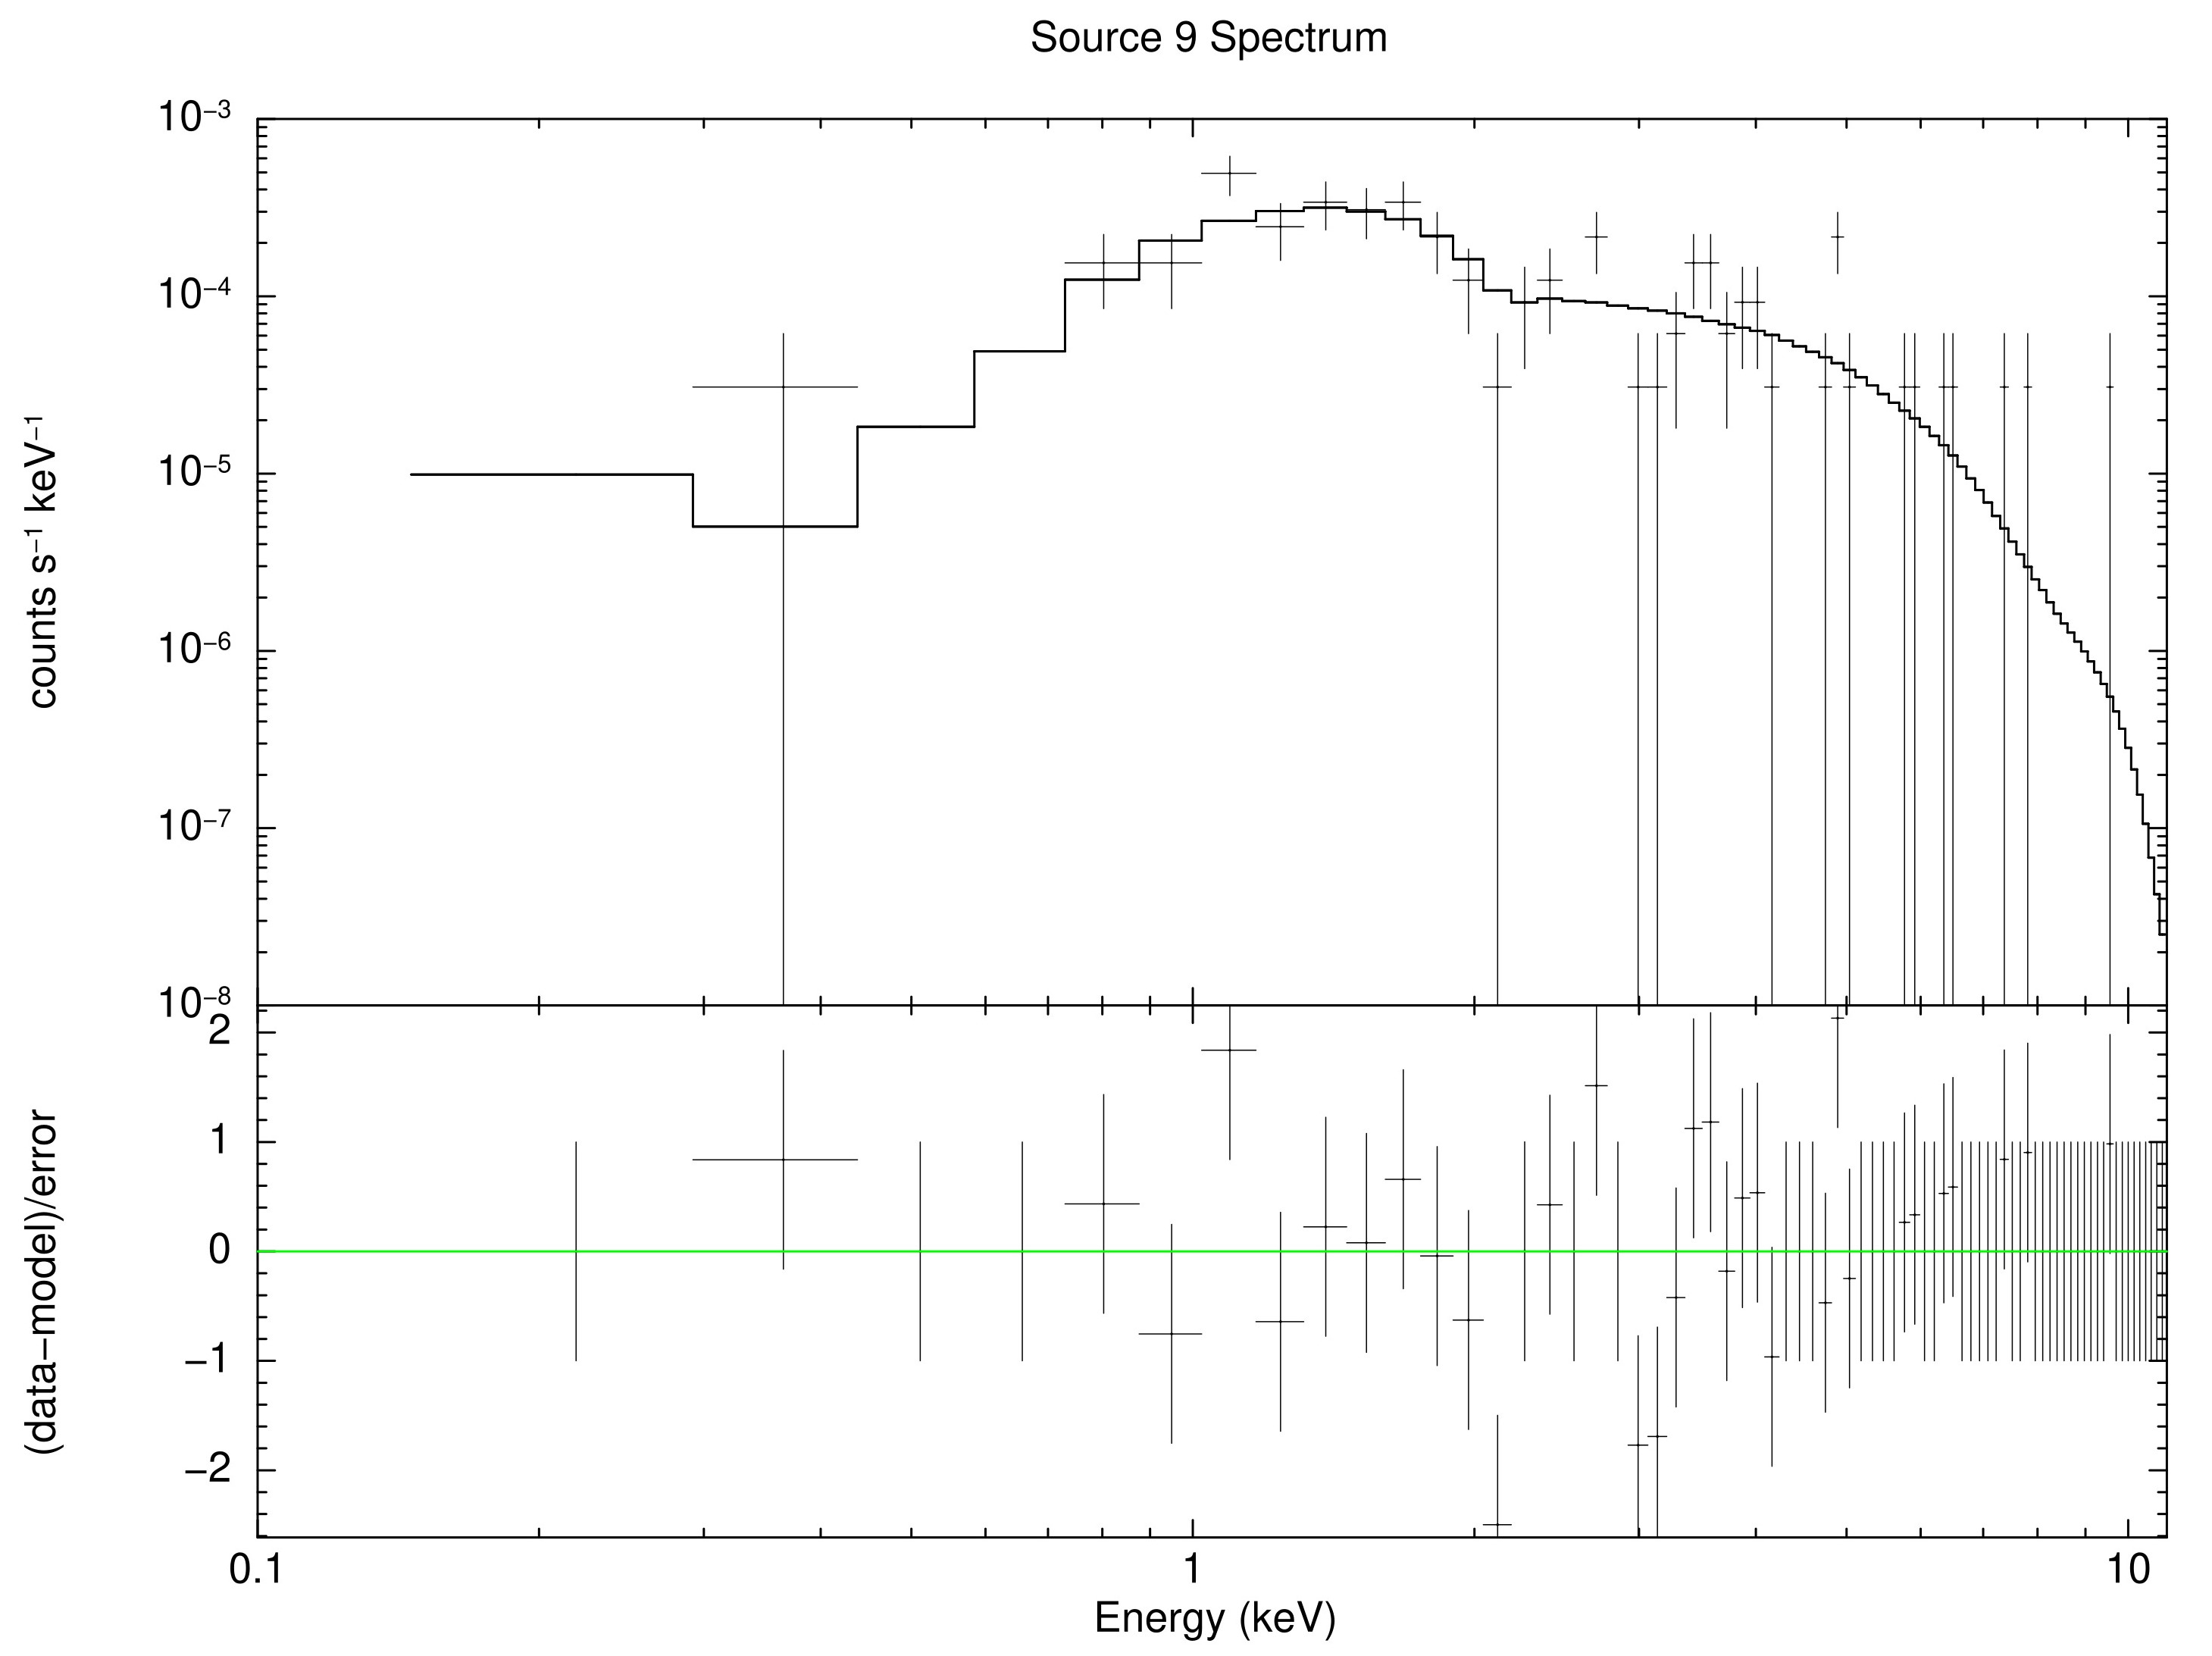
\includegraphics[angle=90, origin=c,width=.45\textwidth]{img/src-9-spectrum.jpg}}\\
    \subfloat[][]{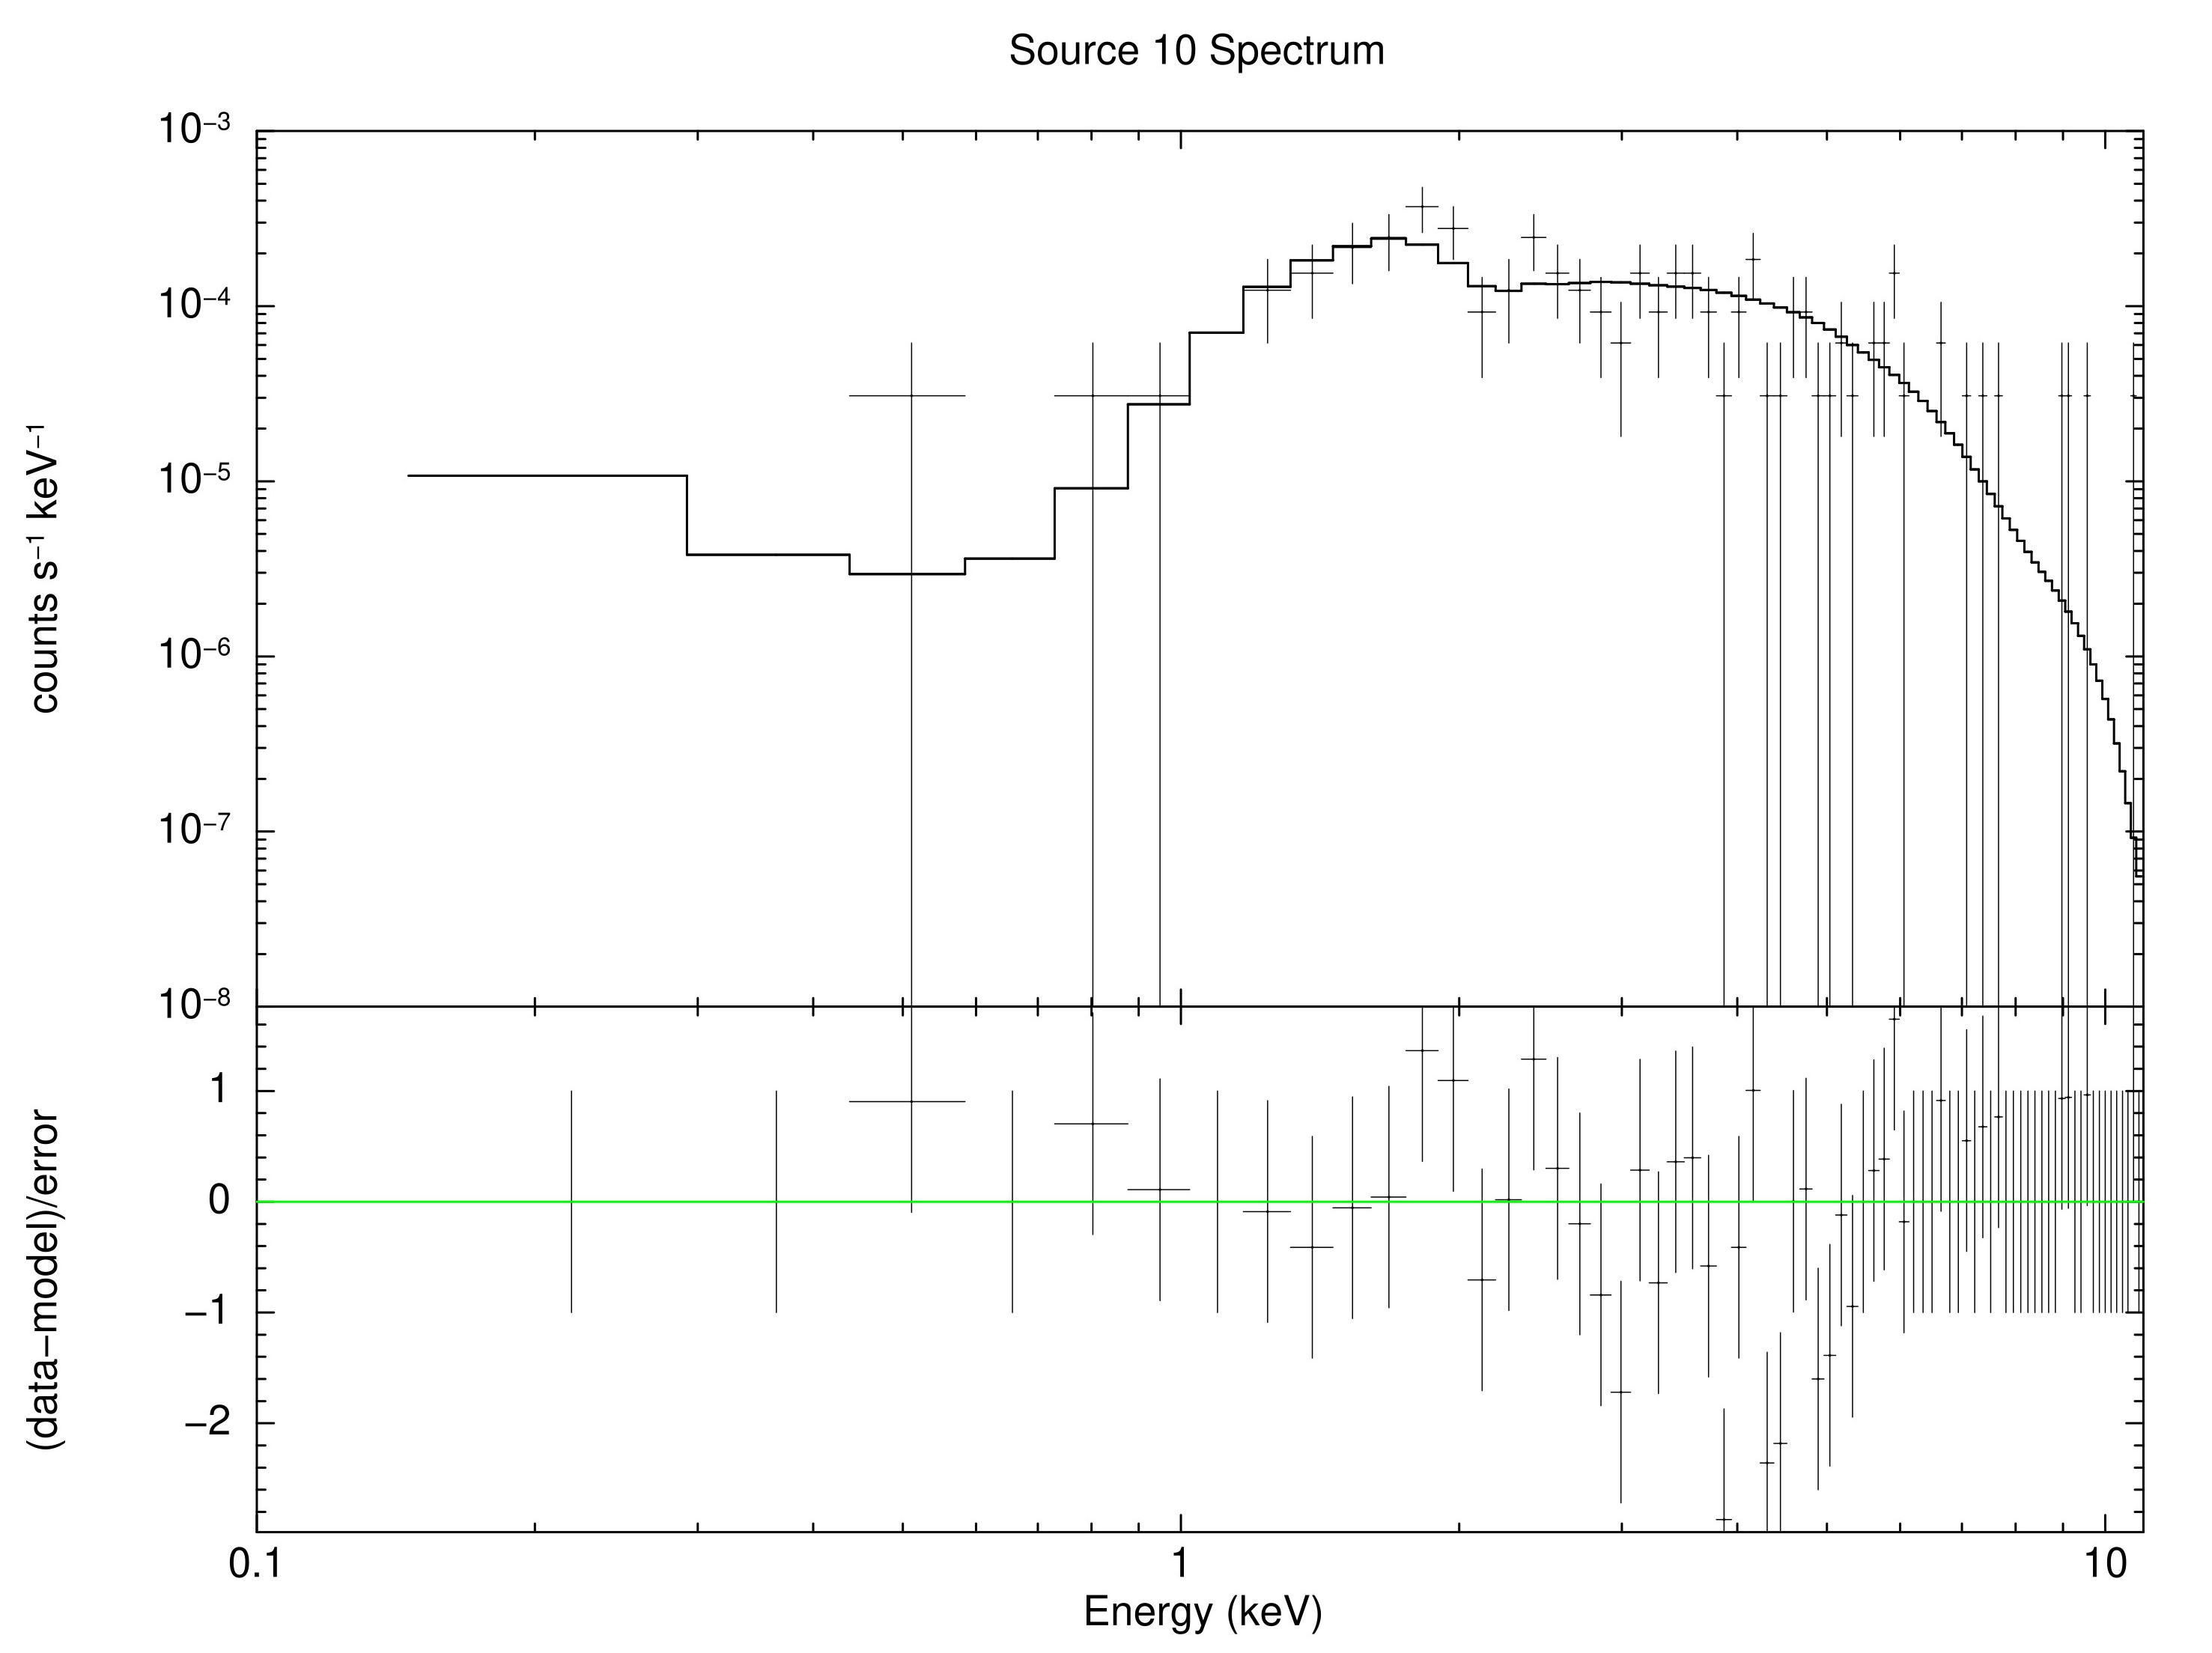
\includegraphics[angle=90, origin=c,width=.45\textwidth]{img/src-10-spectrum.jpg}}\qquad
    \subfloat[][]{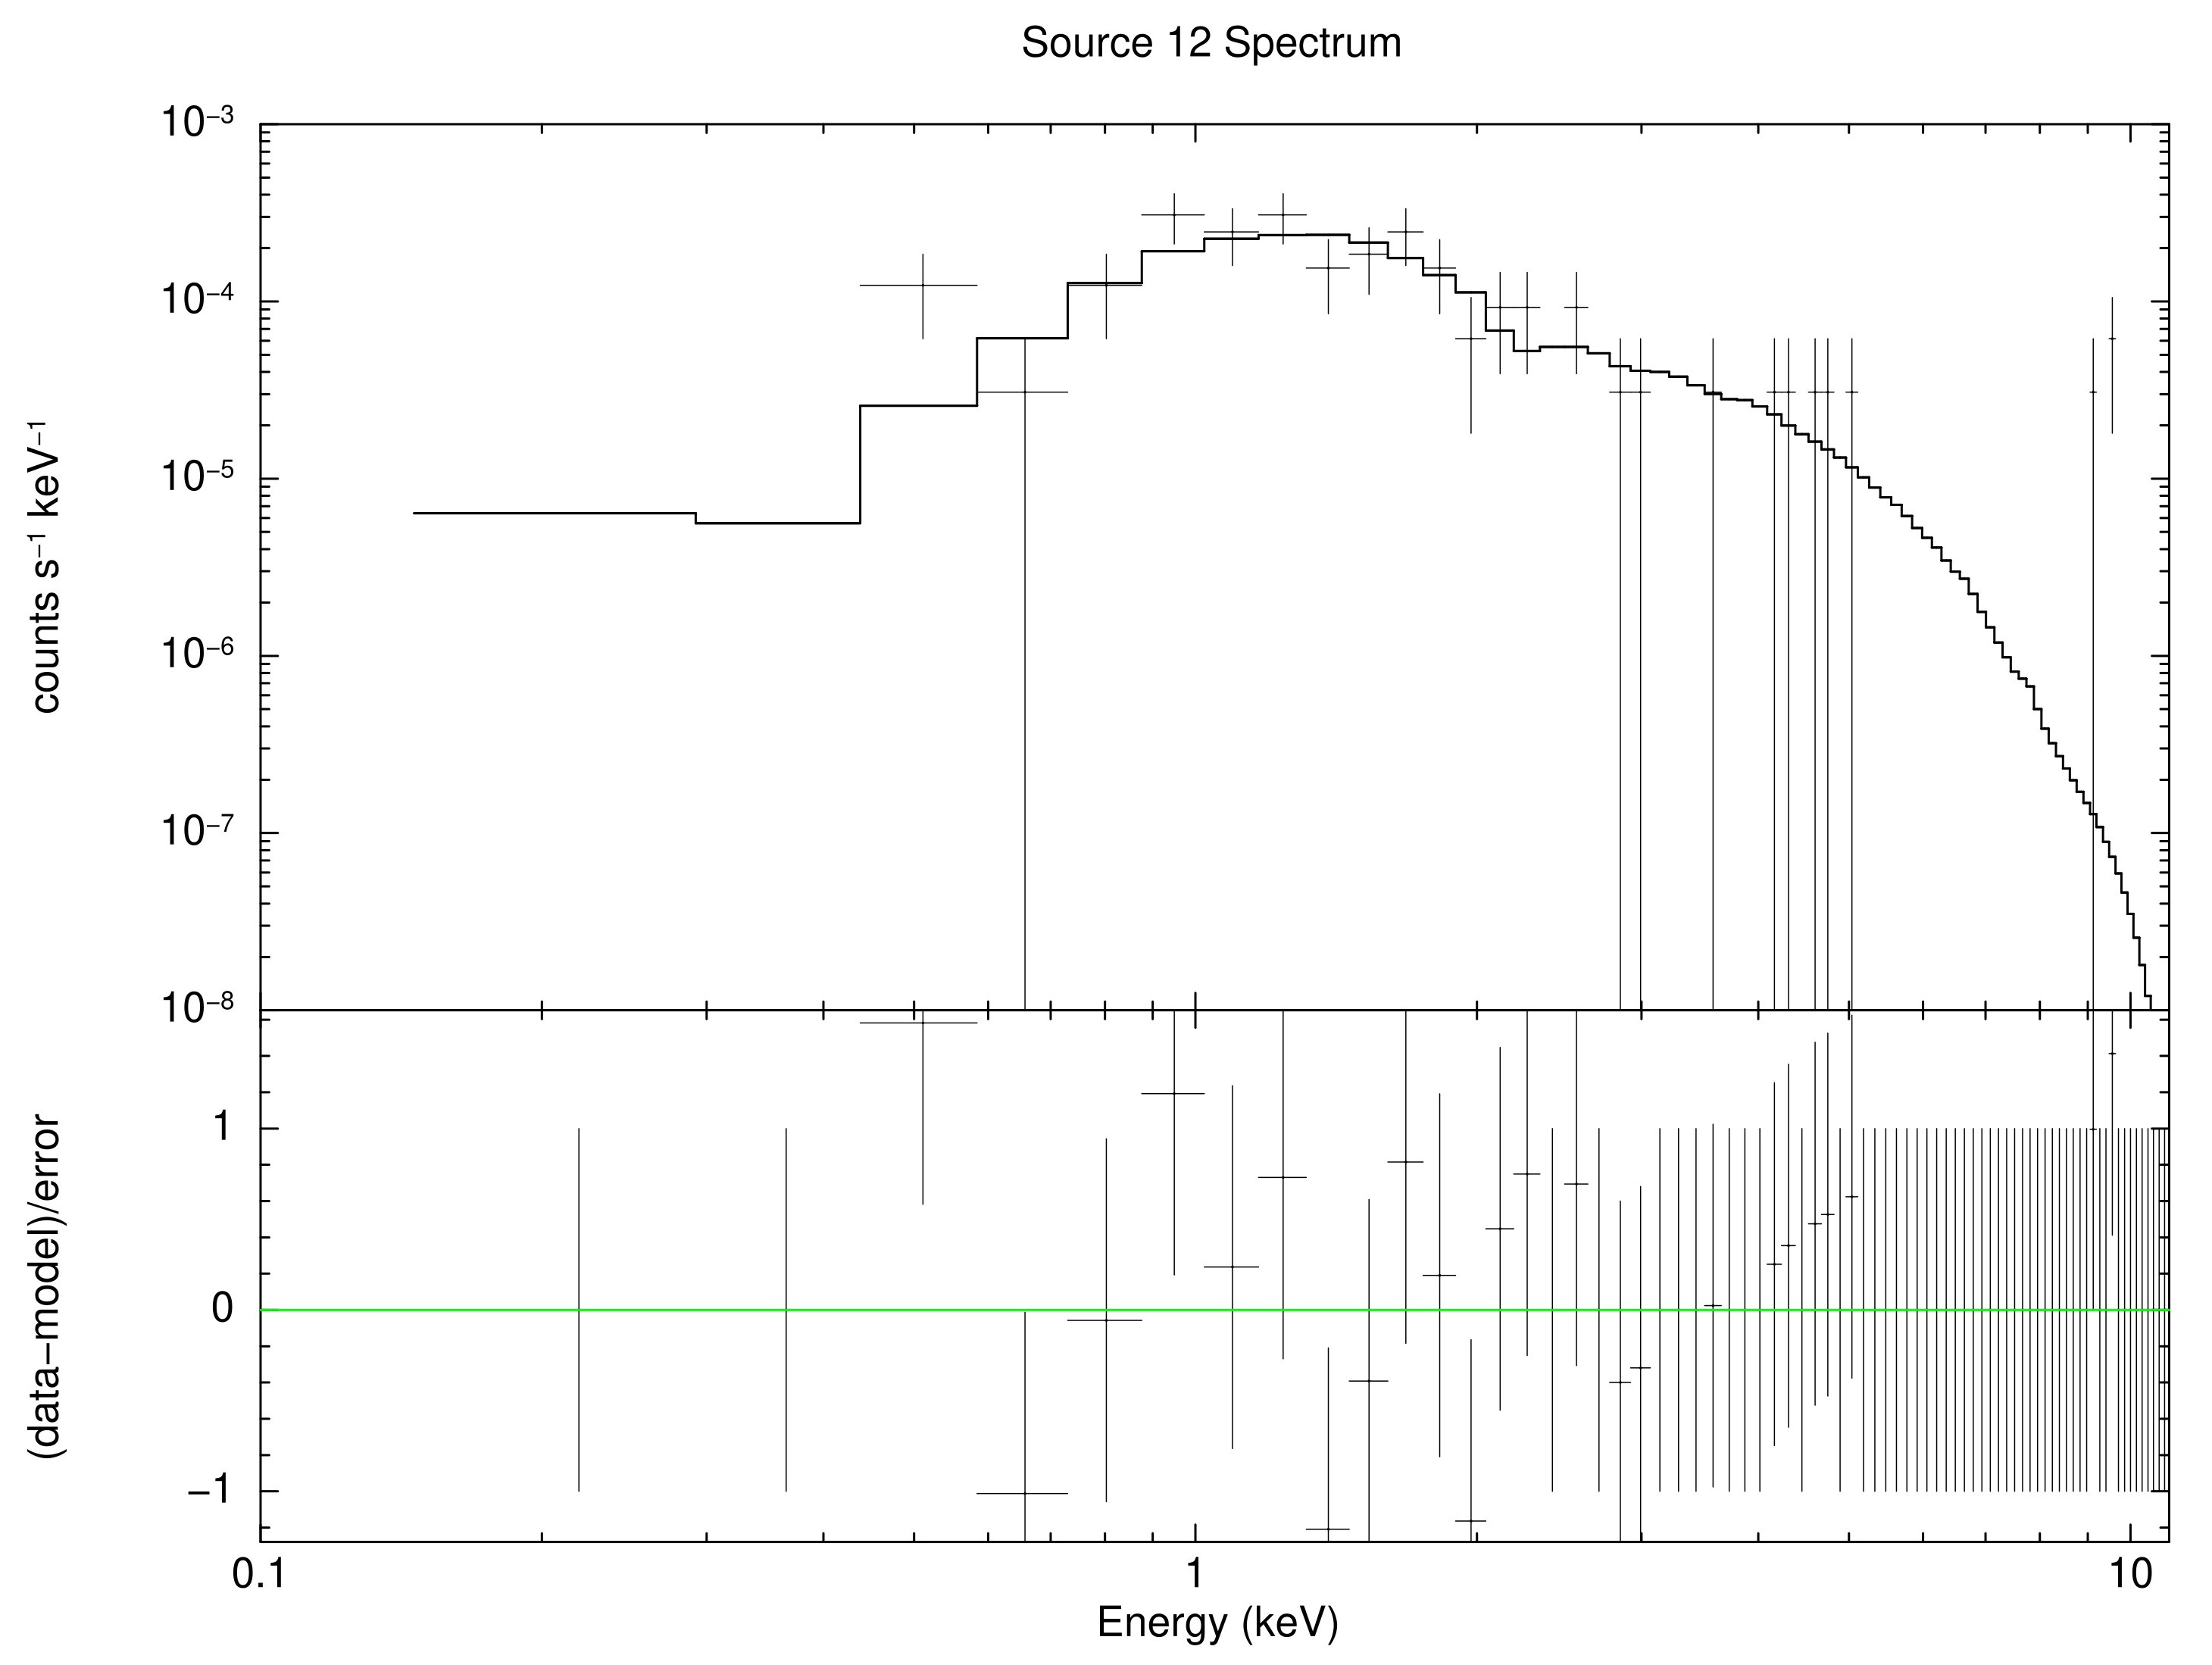
\includegraphics[angle=90, origin=c,width=.45\textwidth]{img/src-12-spectrum.jpg}}
    \caption{}
\end{figure}
\begin{figure}
    \centering
    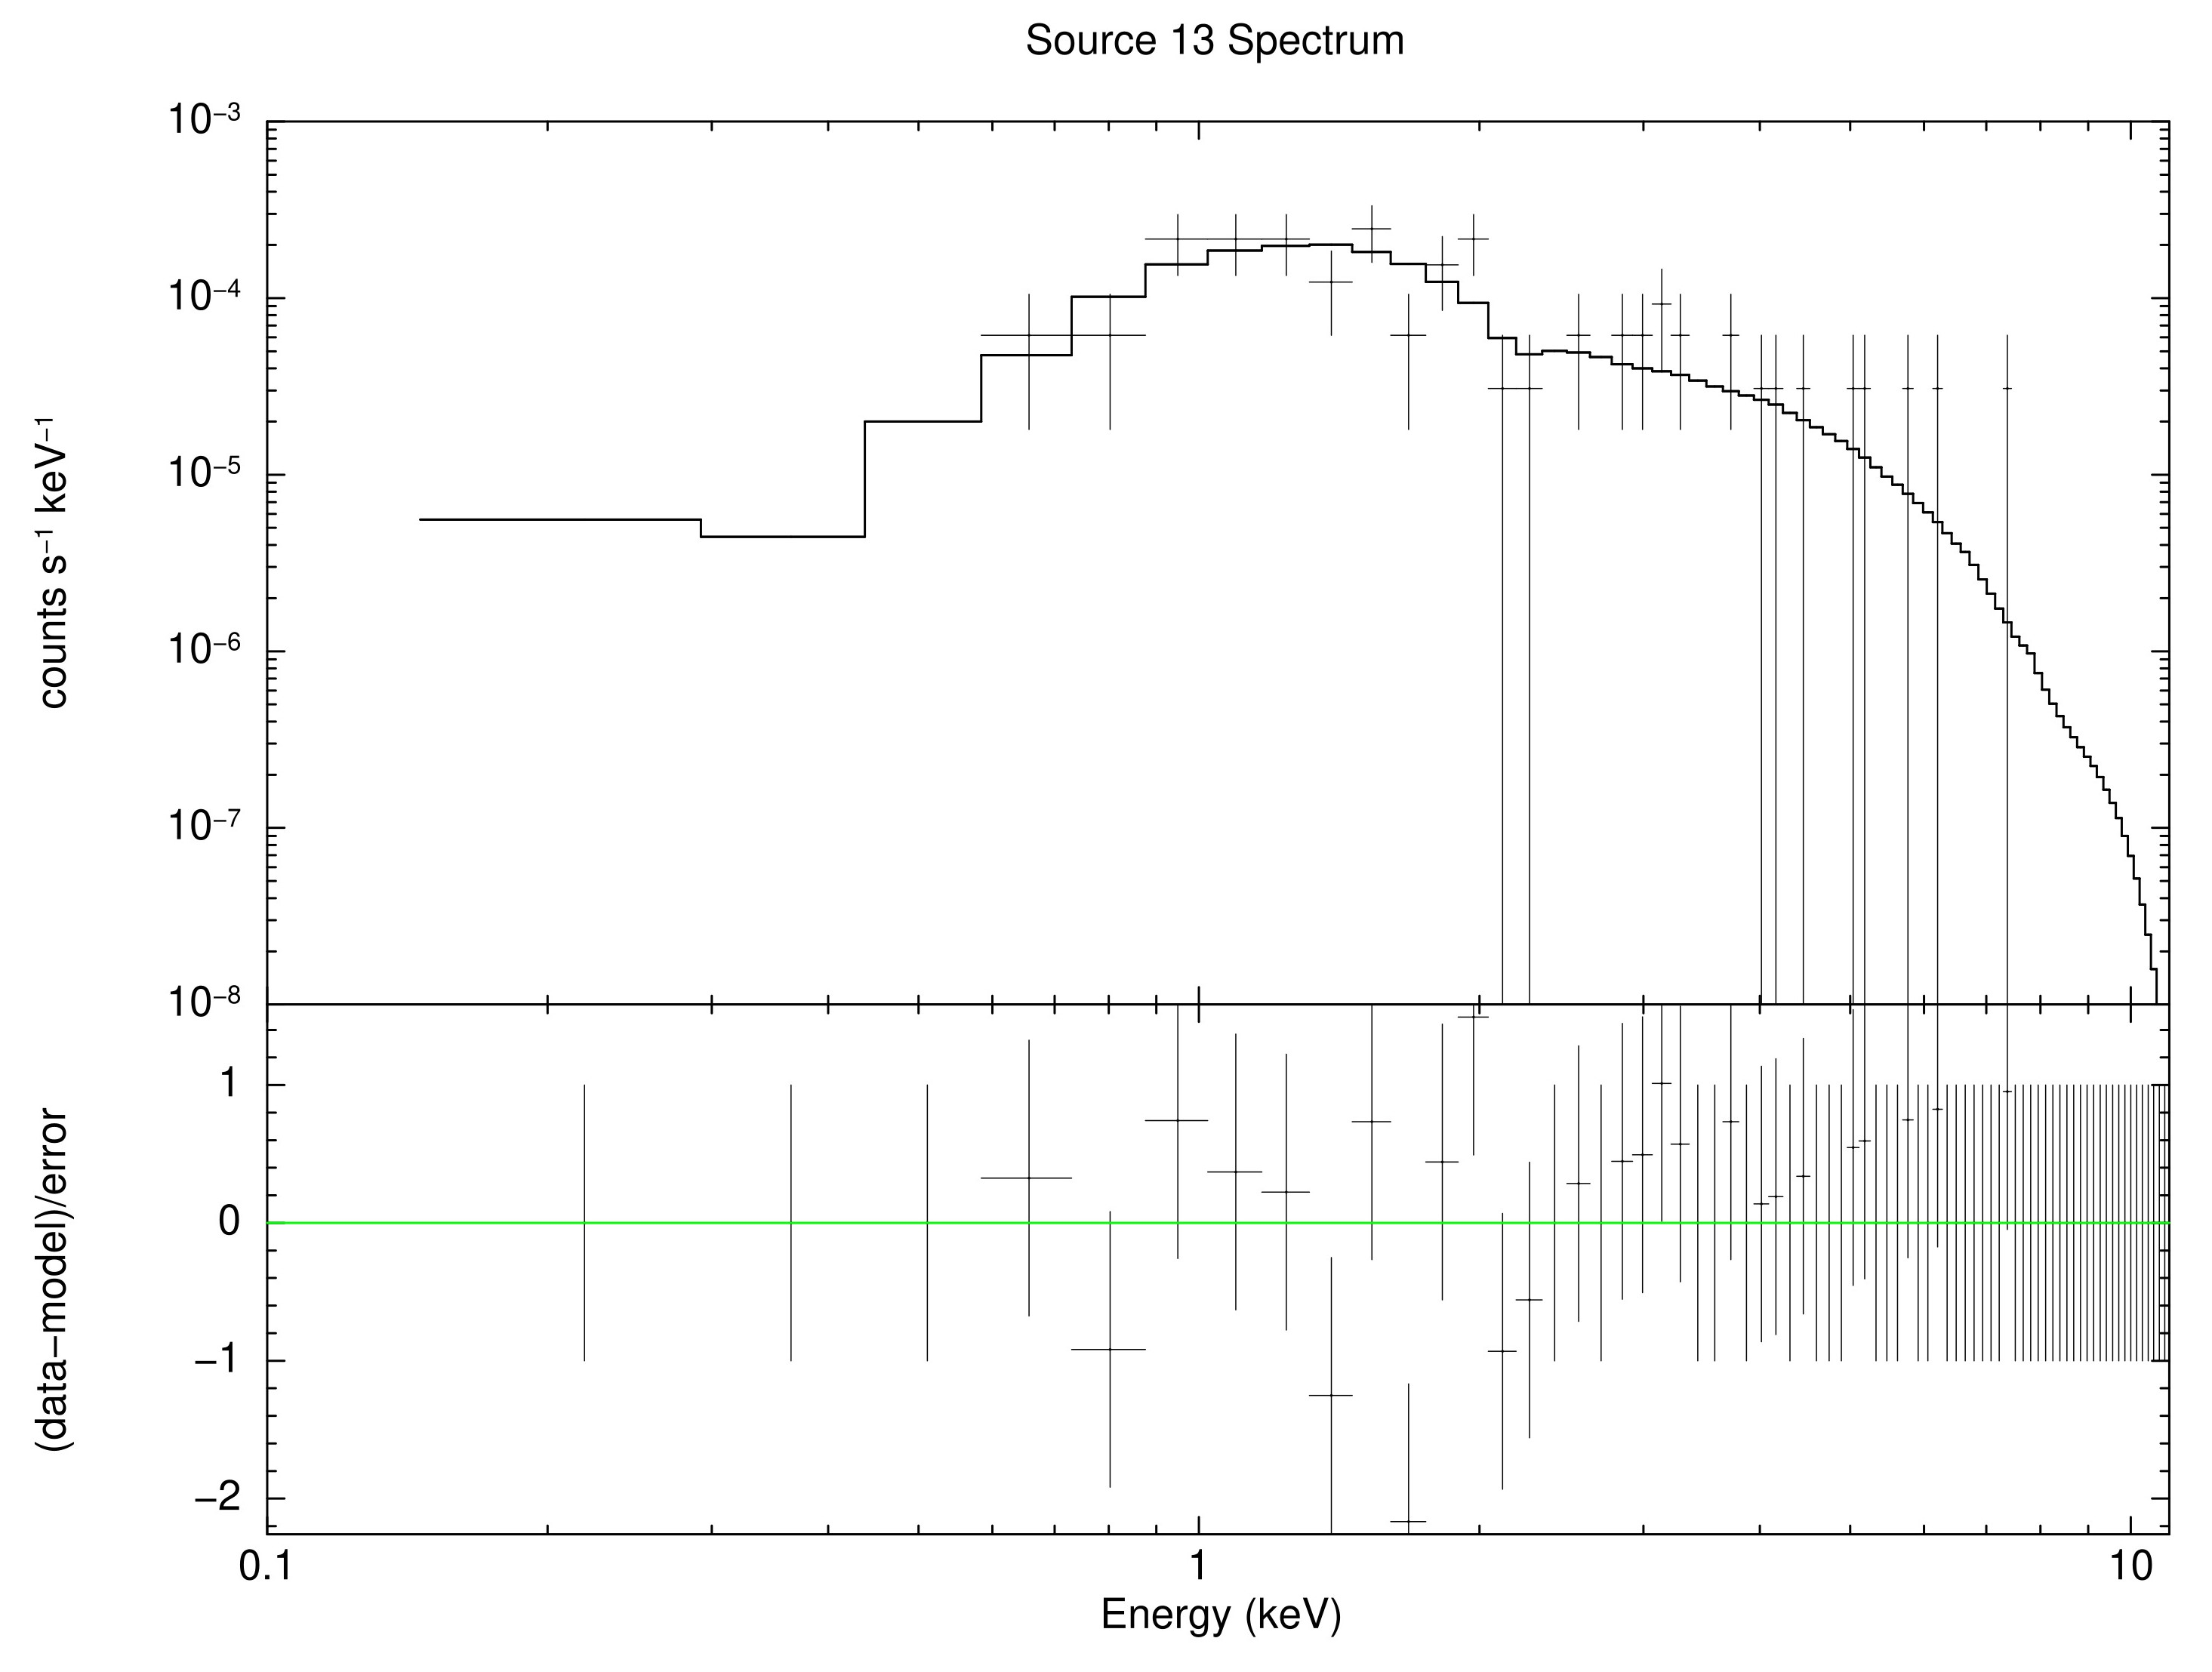
\includegraphics[width=0.85\textwidth, angle=0, origin=c]{img/src-13-spectrum.jpg}
    \caption{}
\end{figure}

\end{document}